\documentclass[11pt,oneside]{amsbook}
\usepackage[T1]{fontenc}
\usepackage{amsmath,amssymb,amsthm,mathtools}
\usepackage[colorlinks=true,linkcolor=blue,citecolor=blue,urlcolor=blue]{hyperref}
\newtheorem{theorem}{Theorem}[chapter]
\newtheorem{proposition}[theorem]{Proposition}
\newtheorem{lemma}[theorem]{Lemma}
\theoremstyle{definition}
\newtheorem{definition}[theorem]{Definition}
\theoremstyle{remark}
\newtheorem{remark}[theorem]{Remark}
\setcounter{tocdepth}{1}
\title{Kravchuk Encyclopedia\\ A Working Book Skeleton}

\date{}
\usepackage{graphicx}
\begin{document}
\frontmatter
\maketitle
% Dedicated portrait page immediately after the title page.
\clearpage
\thispagestyle{empty}
\null\vfill
\begin{center}
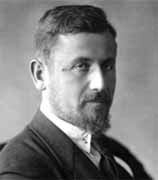
\includegraphics[width=0.42\textwidth,height=0.58\textheight,keepaspectratio]{figures/kravchuk-portrait.jpg}

\vspace{1.2em}
{\large Mikhail Kravchuk (1892--1942)\par}
\vspace{0.6em}
{\small Portrait source: MacTutor History of Mathematics Archive,\par
University of St Andrews.\par}
\end{center}
\vfill\null
\clearpage

\chapter*{Editorial Preface}
This editable skeleton follows the eighteen main topics and appendix program in Section 6.1 of the supplied article source, \texttt{KravFeinsKocik.tex}. Additional headings from the supplied archived website, \texttt{Kravchuk.zip}, have been placed within the closest corresponding chapters. The archived introduction now appears as the first numbered chapter; the eighteen topical chapters follow it. The contents preserve the original program rather than impose a new textbook sequence.

This remains a working encyclopedia, not a completed literature review. Developed sections now include finite matrix identities, source-based representation material, martingales, orthogonality, and Gaussian--Krawtchouk summation. Remaining gaps carry visible uppercase NEEDS TO BE DONE notices, including narrower unfinished tasks within otherwise developed sections. Spectral-asymptotic working material remains explicitly distinguished from proved identities. The source register below separates supplied materials, editorial derivations, and bibliography records awaiting independent verification.

The title retains ``Kravchuk'' while the polynomial notation uses the conventional spelling ``Krawtchouk.'' Historical names and original terminology should be checked as chapters are developed. In particular, the operator symbols $A$, $K$, $\Lambda$, and $T$ require definitions from their original source contexts before they are used interchangeably.
\chapter*{Notation and Conventions}
Throughout the starter material, $K_n(j;N)$ is defined by the ordinary generating function, $k_n(N-2j,N)=n!K_n(j;N)$, $\Phi_N=(K_n(j;N))$, $B_N=\operatorname{diag}(\binom Nj)$, and $S_N=\Phi_NB_N$. All matrix indices begin at zero. In the standard column-vector basis,
$R_Ne_j=(N-j)e_{j+1}$, $L_Ne_j=je_{j-1}$, and $A_N=R_N+L_N$.
The diagonal matrix $\Lambda_N$ has entries $N-2j$.
These conventions, including the distinction between $\Phi_N$ and
$S_N$, are developed in Sections~\ref{sec:finite-sl2-matrices},
\ref{sec:matrix-Phi-definition}, and~\ref{sec:matrix-S-definition}.
Appendix~\ref{app:matrix-tables} contains verified examples for
$N=2,3,4,5,7,8$. Physicists' and probabilists' Hermite normalizations must be explicitly distinguished. Binomial coefficients outside their usual integer range vanish.

\section*{Dictionary for the integrated Kocik article}
The notation of \cite{KocikFeynman} is translated rather than adopted.
Its total order $n$, row $p$ and column $q$ become our $N,n,j$;
its Krawtchouk matrix $K$ becomes $\Phi_N$, its Kac matrix $M$ becomes
$A_N$, and its eigenvalue matrix becomes $\Lambda_N$.
The source's diagonal binomial metric $\Gamma$ becomes $B_N$;
its Pascal matrix $B$ becomes the already established $P_N$.
The source's operator $N=[L,R]$ becomes $\Lambda_N$ on the fixed-order
space, not the scalar order $N$. We use the ordinary commutator
$[X,Y]=XY-YX$, distinguishing it from the source's half-commutator.
The symbols $\Phi_N$, $S_N=\Phi_NB_N$, and $U_N$ retain their distinct
meanings throughout. The parity matrix is $D_N$; powers-of-two weights
in Pascal coordinates are $W_N$.


\section*{Preferred conventions for the newly supplied summary papers}
For general-parameter transform material we retain the supplied
\texttt{KravPQ.tex} notation $K_n(x,N)$ with exponential coefficients.
For the sums material we retain $\phi^N_{nj}$ and its symmetric
specialization $\Phi^N_{nj}$ from \texttt{KravSums.tex}.
Chapter~\ref{chap:pq-source-summary} supplies the parameter interchange,
factorial scaling, and dictionary to earlier chapters. Previously established
symmetric notation is retained there to avoid silently altering formulas.

\tableofcontents
\mainmatter
\chapter{Introduction}
\label{ch:introduction}
\begin{flushright}
\texttt{Omnibus ex nihilo ducendis sufficit unum.}\\
\emph{``To make all things from nothing, unity suffices.''}\\
\textbf{Leibniz}
\end{flushright}
\begin{center}
\textbf{The Kravchuk Encyclopedia}\\
\emph{Ph. Feinsilver and J. Kocik}
\end{center}
So it is written on a medal entitled \emph{Imago Creationis} and designed by Leibniz to \emph{``exhibit to posterity in silver''} his discovery of the binary system.

\medskip
\noindent\textbf{Note on spellings.}
Since the original articles appeared in the French Academy journal \emph{C.R.A.S.}, the French spelling Krawtchouk was used and has been generally adopted. We will use with equal propriety the English spelling Kravchuk, which, in fact, we encourage in the current context.

\medskip
This is the beginnings of a `Kravchuk Encyclopedia'. From the outline presented here, as the project develops, the gaps will gradually be filled in. We hope that you will find lots of interesting material in this work.

% Editorial addition; distinct from the archived introduction.
\section{Mikhail Kravchuk (1892--1942): life and mathematical legacy}
\label{sec:kravchuk-biography}



Mikhail Kravchuk, also known as Mykhailo Pylypovych Kravchuk, was a
Ukrainian mathematician whose work ranged across algebra, differential
and integral equations, probability, and mathematical statistics. He was
born on 27 September 1892 in Chovnitsy, in Volyn, in what is now Ukraine,
and died on 9 March 1942 in a Soviet forced-labour camp in Kolyma.
The biographical outline here draws on the MacTutor History of Mathematics
Archive and the institutional biography maintained by the Institute of
Mathematics of the National Academy of Sciences of Ukraine.\footnote{MacTutor
History of Mathematics Archive, University of St Andrews,
``Mykhailo Pilipovich Krawtchouk,''
\url{https://mathshistory.st-andrews.ac.uk/Biographies/Krawtchouk/};
Institute of Mathematics, National Academy of Sciences of Ukraine,
``Kravchuk Mikhail Pilipovich (1892--1942),''
\url{https://www.imath.kiev.ua/famous?n=kravchuk&lang=en}.
These are secondary biographical accounts, not archival documents.}

\subsection*{Education and scientific career}
Kravchuk's family moved to Lutsk in 1901. He completed his schooling there
with a gold medal in 1910 and entered the University of Kyiv, then
St Vladimir University, graduating in 1914. His early research included
commuting matrices. After the upheavals of the First World War and the
subsequent revolutionary and civil-war years, he combined university
teaching with work in schools. He defended his doctoral dissertation in
1924 and received the title of professor in 1925. His work on matrices,
bilinear forms, and linear transformations was an important part of this
early development.

In 1929 he was elected a full member of the Ukrainian Academy of Sciences.
He taught at the Kyiv Polytechnic Institute and served as head of its
mathematics chair. The Institute of Mathematics identifies him as one of
its founders. His activity was not confined to research: he helped develop
Ukrainian-language mathematical education and terminology, wrote teaching
materials, and supported the training of younger mathematicians.

\subsection*{The polynomials and the scope of his work}
The orthogonal polynomials bearing his name were introduced in 1929.
They are associated with the binomial distribution, providing the
historical starting point for the finite orthogonality and transform
identities developed in this Encyclopedia. Their subsequent uses in
coding theory, finite transforms, and algebraic constructions belong to
the later development of the subject; they should not all be attributed
to Kravchuk himself.

Although these polynomials are now his most familiar mathematical legacy,
his research was considerably broader. It included matrix theory, the
method of moments, differential and integral equations, probability,
statistics, and questions in mathematical education. This wider setting
is particularly relevant here: the interplay between matrices,
orthogonality, and operator methods is not merely an accidental grouping
of topics under one name.

\subsection*{Persecution, death, and rehabilitation}
Kravchuk was arrested in 1938 during Stalin's purges and sentenced on
political charges to twenty years of imprisonment. He was sent to Kolyma,
where he died in 1942, aged forty-nine. MacTutor describes coercion and
threats against his family during the proceedings. He was posthumously
rehabilitated in 1956. His membership in the Ukrainian Academy of Sciences
was restored in 1992. These events are essential to an account of his
career: its abrupt end was a consequence of political repression, not a
natural conclusion to his scientific work.\footnote{For the account of
his persecution, rehabilitation, and restoration of Academy membership,
see the MacTutor biography cited above.}

\subsection*{Names and conventions in this Encyclopedia}
The spellings \emph{Kravchuk}, \emph{Krawtchouk}, and \emph{Krawtschuk}
reflect different transliterations. MacTutor notes that \emph{Krawtchouk}
was the spelling used in his French-language papers. We retain
\emph{Kravchuk} in the Encyclopedia's title and historical discussion,
while respecting \emph{Krawtchouk} in established mathematical terminology,
source titles, and quotations. The first names \emph{Mikhail} and
\emph{Mykhailo} likewise occur in the biographical literature. These
variants refer to the same mathematician.

\medskip
\noindent\emph{Editorial provenance.} This sourced biographical section
is a later addition to the Encyclopedia. It is not part of the archived
2001 introduction, whose wording and attribution are retained separately.


\section*{Starting points}
The original introduction offered the following entry points, now represented within this book:
\begin{itemize}
\item \emph{First View}: see Section~\ref{sec:1-5}.
\item \emph{Krawtchouk Matrices}: see Section~\ref{sec:1-4}.
\item \emph{Kravchuk Polynomials}: see Section~\ref{sec:1-2}.
\item \emph{Twistons}: see Section~\ref{sec:9-6}.
\item \emph{Other Examples}: reserved for future additions to the introductory material.
\end{itemize}
For transforms, see Chapter~\ref{ch:14}. The complete table of contents replaces the original website's \emph{To Contents} link.

\section*{Archival note}
This chapter transcribes the substantive text of \texttt{Kravchuk/Introduction.html} in the supplied website archive. The displayed author attribution and the historical wording above are retained from that source; they do not assign authorship of later editorial additions. Its modification footer records July 28, 2001. The historical claims and quotation are reproduced as source text and have not been independently verified for this skeleton.

The original page also linked to an interactive K-transform form and a bibliographic search database. Those were website services rather than book text; they are recorded here as archival resources, not represented as functioning services. Navigation has been adapted to book cross-references.

\chapter{Pascal's Triangle}
\label{ch:1}
\section{Pascal's triangle and binomial identities}
\label{sec:1-1}
Choosing an $n$-element subset of $\{1,\ldots,N\}$ according to whether it contains the last element proves
\begin{equation}\label{eq:pascal-subsets}
\binom Nn=\binom{N-1}n+\binom{N-1}{n-1}.
\end{equation}
We use $\binom Nn=0$ outside $0\le n\le N$. Expanding a product of $N$ factors gives
\[
(1+v)^N=\sum_{n=0}^N\binom Nn v^n.
\]
Taking coefficients in $(1+v)^{a+b}=(1+v)^a(1+v)^b$ gives Vandermonde's identity
\[
\binom{a+b}n=\sum_r\binom ar\binom b{n-r}.
\]
Replacing the second factor by $(1-v)^b$ yields the signed convolution defining $K_n(b;a+b)$ in Section~\ref{sec:1-2}. Thus the first column of the Krawtchouk array is Pascal's row, and its other columns are signed subset counts, not probability distributions.
For example, at $N=3$, the columns for $j=0$ and $j=1$ are respectively $(1,3,3,1)^T$ and $(1,1,-1,-1)^T$.

\section{Krawtchouk polynomials}
\label{sec:1-2}
For $0\leq n,j\leq N$, define the symmetric Krawtchouk polynomial values by
\begin{equation}\label{eq:gen}
(1+v)^{N-j}(1-v)^j=\sum_{n=0}^N K_n(j;N)v^n.
\end{equation}
Hence
\[
K_n(j;N)=\sum_r(-1)^r\binom jr\binom{N-j}{n-r}.
\]
Binomial coefficients outside their usual range are understood to vanish.
In centered coordinates $x=N-2j$, write
\[
(1+v)^{(N+x)/2}(1-v)^{(N-x)/2}
=\sum_{n=0}^N\frac{v^n}{n!}k_n(x,N).
\]
Thus $k_n(N-2j,N)=n!K_n(j;N)$.

\section{Generating functions}
\label{sec:1-3}
Write $x=N-2j$ and use the generating function in \eqref{eq:gen}. Logarithmic differentiation gives the polynomial identity
\[
(1-v^2)\frac{\partial G_{N,j}}{\partial v}=(x-Nv)G_{N,j}.
\]
Coefficient comparison, with $K_{-1}=0$, yields
\[
(n+1)K_{n+1}(j;N)=xK_n(j;N)-(N-n+1)K_{n-1}(j;N).
\]
In particular,
\[
K_0=1,\qquad K_1=x,\qquad K_2=\frac{x^2-N}{2},\qquad
K_3=\frac{x^3-(3N-2)x}{6}.
\]
The factorial-scaled polynomials are $k_n=n!K_n$, so their leading coefficient as polynomials in $x$ is one. This is why factorials must be retained when passing between ordinary and exponential generating functions.
At the endpoints,
\[
K_n(0;N)=\binom Nn,\qquad K_n(N;N)=(-1)^n\binom Nn.
\]
Moreover, $G_{N,N-j}(v)=G_{N,j}(-v)$, giving $K_n(N-j;N)=(-1)^nK_n(j;N)$. These are fixed-order identities, distinct from the cross-order construction of Section~\ref{sec:1-5}.

\section{Krawtchouk matrices}
\label{sec:1-4}
Set $\Phi_N=(K_n(j;N))_{n,j=0}^N$ and
$B_N=\operatorname{diag}(\binom N0,\ldots,\binom NN)$. Binomial duality is
\[
\binom Nj K_n(j;N)=\binom Nn K_j(n;N).
\]
Consequently $S_N=\Phi_NB_N$ is symmetric. The symmetric transform satisfies
\[
\Phi_N^2=2^NI.
\]
For orientation,
\[
\Phi_1=\begin{pmatrix}1&1\\1&-1\end{pmatrix},\qquad
\Phi_2=\begin{pmatrix}1&1&1\\2&0&-2\\1&-1&1\end{pmatrix}.
\]

\section{First view and cross properties}
\label{sec:1-5}
Write $G_{N,j}(v)=(1+v)^{N-j}(1-v)^j$, as in \eqref{eq:gen}.
Multiplying by $1+v$ or $1-v$ and comparing coefficients gives
\begin{align}
K_n(j;N+1)&=K_n(j;N)+K_{n-1}(j;N),\label{eq:cross-plus}\\
K_n(j+1;N+1)&=K_n(j;N)-K_{n-1}(j;N).\label{eq:cross-minus}
\end{align}
Here $0\leq j\leq N$, and coefficients outside $0\leq n\leq N$
vanish at order $N$. Adding and subtracting yields the inverse cross rules
\begin{align*}
K_n(j;N+1)+K_n(j+1;N+1)&=2K_n(j;N),\\
K_n(j;N+1)-K_n(j+1;N+1)&=2K_{n-1}(j;N).
\end{align*}
These are cross-order identities: the order parameter must not be
suppressed when they are used to construct successive tables.
For example, $K_2(1;3)=-1$ and $K_1(1;3)=1$ give
$K_2(1;4)=0$ and $K_2(2;4)=-2$.

There is also a fixed-order local relation. If
\[
\begin{pmatrix}a&b\\c&d\end{pmatrix}
=\begin{pmatrix}K_n(j;N)&K_n(j+1;N)\\
K_{n+1}(j;N)&K_{n+1}(j+1;N)\end{pmatrix},
\]
then $-a+c=b+d$. Indeed,
$(1-v)G_{N,j}=(1+v)G_{N,j+1}$.
Column reversal and row reversal are instead the fixed-order
symmetries proved in Section~\ref{sec:8-1}; these should be distinguished
from the cross-order rules above. Compare \cite[Appendix~C]{KocikFeynman}.


\chapter{Random Walks}
\label{ch:2}
\section{Paths and path integrals}
\label{sec:2-1}
Consider length-$N$ binary paths $w=(w_1,\ldots,w_N)$, where
$w_a\in\{0,1\}$ and $|w|=\sum_aw_a$ is the endpoint coordinate.
Fix $j$ distinguished steps and assign the signed weight
\[
\omega_j(w)=(-1)^{w_1+\cdots+w_j}.
\]
The particular first-$j$ choice is inessential; any fixed subset of $j$
steps gives the same endpoint sums. A path with endpoint $n$ and $r$
right steps among the distinguished steps has weight $(-1)^r$.
There are $\binom jr\binom{N-j}{n-r}$ such paths, so
\begin{equation}\label{eq:signed-path-Krawtchouk}
\sum_{|w|=n}\omega_j(w)
=\sum_r(-1)^r\binom jr\binom{N-j}{n-r}
=K_n(j;N).
\end{equation}
This is a path interpretation of the coefficient formula in
Section~\ref{sec:1-2}, not a new definition. For $j=0$ it counts ordinary
paths and gives $\binom Nn$; for $j>0$, cancellation produces signed
entries of column $j$ of $\Phi_N$. For instance, $N=4$, $j=2$ gives
endpoint sums $(1,0,-2,0,1)$.

The signed Galton-board construction of \cite[Section~6]{KocikFeynman}
is an elementary analogue of a sum over paths. Its weights are not
probabilities. In quantum mechanics one sums amplitudes before taking
an appropriately normalized absolute square; a physical unitary model
requires more structure than this combinatorial identity. The unsigned
walk and the stochastic Ehrenfest transition operator should likewise
not be identified with a unitary evolution.


\subsection{Weighted paths and the two-parameter deformation}
\label{sec:weighted-path-deformation}
Over a commutative ring, define a separate coefficient array
\[
\mathcal K_n(j;N;\alpha,\beta)
=[v^n](1+\alpha v)^{N-j}(1+\beta v)^j.
\]
A consistent path rule gives every left step weight $1$, and a right
step weight $\beta$ at each of $j$ distinguished times and $\alpha$ at
all other times. Thus
\[
\mathcal K_n(j;N;\alpha,\beta)
=\sum_r\binom jr\binom{N-j}{n-r}\beta^r\alpha^{n-r}.
\]
This recovers $K_n(j;N)$ at $(\alpha,\beta)=(1,-1)$ without changing
its normalization. Coefficient comparison gives
\begin{align*}
\mathcal K_n(j;N+1)&=\mathcal K_n(j;N)+\alpha\mathcal K_{n-1}(j;N),\\
\mathcal K_n(j+1;N+1)&=\mathcal K_n(j;N)+\beta\mathcal K_{n-1}(j;N).
\end{align*}
For adjacent entries $\begin{pmatrix}a&b\\c&d\end{pmatrix}$ in this
array, $\beta a+c=\alpha b+d$.
These identities require no division by $\alpha-\beta$ and remain valid
when parameters coincide or are not invertible.

\begin{remark}[A discrepancy in the source's path rule]
The displayed generating function of \cite[Section~6.2]{KocikFeynman}
is the one used here. However, the preceding prose assigns left/right
weights $\alpha,\beta$ only at the $j$ distinguished times, and weights
$1,1$ elsewhere. That different rule produces
$(1+v)^{N-j}(\alpha+\beta v)^j$, not the displayed generating function.
We retain the displayed coefficient array and specify the compatible
rule explicitly. No stochastic normalization, orthogonality, or
involution property is asserted for arbitrary parameters.
\end{remark}

\section{$A$, $K$, and $\Lambda$}
\label{sec:2-2}
For the symmetric walk on $\{0,\ldots,N\}$, use column vectors for
state distributions and the zero-based standard basis $e_j$. Put
\[
A_Ne_j=(N-j)e_{j+1}+je_{j-1},\qquad
\Lambda_N=\operatorname{diag}(N,N-2,\ldots,-N),
\]
with endpoint terms omitted. In this section the matrix symbol $K$
is explicitly defined to mean $\Phi_N=(K_n(j;N))_{n,j=0}^N$.
It is not a single polynomial $K_n$ or the symmetric matrix
$S_N=\Phi_NB_N$.

\subsection{Intertwining and diagonalization}
Writing $G_j(v)=(1+v)^{N-j}(1-v)^j$, differentiation gives
\[
(1-v^2)G_j'(v)=(N-2j-Nv)G_j(v).
\]
Equating coefficients yields
\[
(N-n+1)K_{n-1}(j;N)+(n+1)K_{n+1}(j;N)
=(N-2j)K_n(j;N).
\]
The spatial recurrence is
\[
jK_n(j-1;N)+(N-j)K_n(j+1;N)=(N-2n)K_n(j;N).
\]
Absent endpoint terms are zero. In matrix form these identities read
\[
A_N\Phi_N=\Phi_N\Lambda_N,\qquad
\Phi_NA_N=\Lambda_N\Phi_N.
\]
This is the coefficient proof of the master equation; its symmetric-power
interpretation is given in Section~\ref{sec:8-1}.
Since $\Phi_N^2=2^NI$, we obtain
\[
\Phi_N^{-1}=2^{-N}\Phi_N,\qquad
A_N=2^{-N}\Phi_N\Lambda_N\Phi_N.
\]
Column $j$ of $\Phi_N$ is a right eigenvector with eigenvalue $N-2j$;
row $n$ is a left eigenvector with eigenvalue $N-2n$.

\subsection{Transition probabilities}
For $N\geq1$, $T_N=A_N/N$ is column-stochastic. Hence
$p_{t+1}=T_Np_t$ and, for integers $t\geq0$,
\[
T_N^t=2^{-N}\Phi_N(\Lambda_N/N)^t\Phi_N.
\]
The backward operator on column vectors of function values is $T_N^T$,
not $T_N$; its eigenfunctions are $j\mapsto K_n(j;N)$.
The stationary column distribution is
$2^{-N}(\binom N0,\ldots,\binom NN)^T$, the normalized first column
of $\Phi_N$. The eigenvalue $-1$ of $T_N$ expresses period two;
stationarity does not imply convergence from arbitrary initial data.

\subsection{The cases $N=3$ and $N=5$}
For $N=3$,
\begingroup
\small
\setlength{\arraycolsep}{3pt}
\[
A_{3}=\begin{pmatrix}
0 & 1 & 0 & 0 \\
3 & 0 & 2 & 0 \\
0 & 2 & 0 & 3 \\
0 & 0 & 1 & 0
\end{pmatrix}.
\]
\endgroup
\begingroup
\small
\setlength{\arraycolsep}{3pt}
\[
\Lambda_{3}=\begin{pmatrix}
3 & 0 & 0 & 0 \\
0 & 1 & 0 & 0 \\
0 & 0 & -1 & 0 \\
0 & 0 & 0 & -3
\end{pmatrix}.
\]
\endgroup
The transition eigenvalues are $1,\frac{1}{3},- \frac{1}{3},-1$.
For $N=5$,
\begingroup
\small
\setlength{\arraycolsep}{3pt}
\[
A_{5}=\begin{pmatrix}
0 & 1 & 0 & 0 & 0 & 0 \\
5 & 0 & 2 & 0 & 0 & 0 \\
0 & 4 & 0 & 3 & 0 & 0 \\
0 & 0 & 3 & 0 & 4 & 0 \\
0 & 0 & 0 & 2 & 0 & 5 \\
0 & 0 & 0 & 0 & 1 & 0
\end{pmatrix}.
\]
\endgroup
\begingroup
\small
\setlength{\arraycolsep}{3pt}
\[
\Lambda_{5}=\begin{pmatrix}
5 & 0 & 0 & 0 & 0 & 0 \\
0 & 3 & 0 & 0 & 0 & 0 \\
0 & 0 & 1 & 0 & 0 & 0 \\
0 & 0 & 0 & -1 & 0 & 0 \\
0 & 0 & 0 & 0 & -3 & 0 \\
0 & 0 & 0 & 0 & 0 & -5
\end{pmatrix}.
\]
\endgroup
The transition eigenvalues are $1,\frac{3}{5},\frac{1}{5},- \frac{1}{5},- \frac{3}{5},-1$.
The corresponding $R_N$, $L_N$, $\Phi_N$ and $S_N$ tables are in
Appendix~\ref{app:matrix-tables}. Centered and lattice polynomial tables
are in Appendix~\ref{app:polynomial-tables}.

\section{Nonsymmetric walks}
\label{sec:2-3}
% TODO: Develop this section; add verified references, examples, and exercises.

\noindent\textbf{NONSYMMETRIC WALKS NEEDS TO BE DONE.}


\section{Symmetric Krawtchouk matrices and binomial expectations}
\label{sec:2-4}
% TODO: Develop this section; add verified references, examples, and exercises.

\noindent\textbf{SYMMETRIC KRAWTCHOUK MATRICES AND BINOMIAL EXPECTATIONS NEEDS TO BE DONE.}



\section*{Connection to the supplied article sources}
The supplied source \texttt{KravFeinsKocik.tex}, Section~5, develops the
classical Bernoulli random walk and a multivariate extension.
The supplied \texttt{jkhadamard\_Oct\_08\_00.tex}, Section~5, connects
classical random walks with Krawtchouk matrices. Read these alongside
this chapter using the book's ordinary generating-function normalization;
source conventions should not be silently substituted for it.

\chapter{Urn Model}
\label{ch:3}
\section{Markov chains}
\label{sec:3-1}
In the discrete-time Ehrenfest chain, the state $j$ is the number of balls in one of two urns. Moving one uniformly chosen ball gives
\[
(Pf)(j)=\frac{N-j}{N}f(j+1)+\frac jN f(j-1).
\]
The Krawtchouk difference equation gives
\[
P K_n(\cdot;N)=\left(1-\frac{2n}{N}\right)K_n(\cdot;N).
\]
Here $N\geq1$, and terms outside the state space have zero transition coefficient.

\section{Initial and invariant distributions}
\label{sec:3-2}
The invariant distribution is $w_N(j)=2^{-N}\binom Nj$. Detailed balance follows from
\[
w_N(j)\frac{N-j}{N}=w_N(j+1)\frac{j+1}{N}.
\]
The non-lazy discrete-time chain has period two; invariance should not be confused with convergence to equilibrium from every initial distribution.


\section*{Connection to the supplied article sources}
Section~4 (``Ehrenfest urn model'') of the supplied
\texttt{KravFeinsKocik.tex} belongs to this chapter.
The urn state is the Hamming weight of a binary configuration: flipping
a uniformly selected coordinate moves from $j$ to $j+1$ with probability
$(N-j)/N$ and to $j-1$ with probability $j/N$, for $N\geq1$.
In the book's column-vector convention the transition matrix is
$A_N/N$. The tensor-space realization is discussed in Chapter~\ref{ch:9}.

\chapter{Symmetric Functions and Energy}
\label{ch:4}
\section{Elementary symmetric functions and determinants}
\label{sec:4-1}
For scalars $z_1,\ldots,z_N$, the elementary symmetric functions are
\[
e_n(z_1,\ldots,z_N)=\sum_{1\leq a_1<\cdots<a_n\leq N}
z_{a_1}\cdots z_{a_n},\qquad e_0=1.
\]
Each subset occurs once: repeated indices and ordered tuples are excluded.
For $D=\operatorname{diag}(z_1,\ldots,z_N)$,
\begin{equation}\label{eq:elementary-energy-generating}
\det(I+vD)=\prod_{a=1}^N(1+z_av)
=\sum_{n=0}^N e_n(z_1,\ldots,z_N)v^n.
\end{equation}
If $z_a=\epsilon_a\in\{+1,-1\}$ and precisely $j$ signs are negative,
comparison with the defining generating function \eqref{eq:gen} gives
\begin{equation}\label{eq:sign-energy-Krawtchouk}
e_n(\epsilon_1,\ldots,\epsilon_N)=K_n(j;N).
\end{equation}
Thus the order-$n$ interaction energy depends only on the number of
negative signs, not their positions. The first two nonconstant energies are
\[
e_1=N-2j,\qquad e_2=\frac{(N-2j)^2-N}{2}.
\]
These are ordinary coefficient values, not the factorial-scaled centered
polynomials: $k_n(N-2j,N)=n!e_n$.
The twiston interpretation is given in Section~\ref{sec:9-6}; the signed-path
interpretation in Section~\ref{sec:2-1} gives the same coefficients by a
different combinatorial construction. See also \cite[Sections~1 and~5]{KocikFeynman}.

\section{Traces on Grassmann algebras}
\label{sec:4-2}
Let $V$ have dimension $N$ and let $T:V\to V$ be linear. On the $n$th exterior power define
\[
(\bigwedge^n T)(v_1\wedge\cdots\wedge v_n)
=Tv_1\wedge\cdots\wedge Tv_n.
\]
The trace of this induced map is the sum of the principal $n\times n$ minors of $T$. Consequently,
\begin{equation}\label{eq:exterior-trace-determinant}
\det(I+vT)=\sum_{n=0}^N v^n\operatorname{tr}(\bigwedge^n T).
\end{equation}
Indeed, in an exterior basis indexed by subsets, the diagonal entry indexed by a subset is precisely its principal minor; the determinant expansion gives the same coefficients. This argument does not require diagonalizability.
For a sign operator $D$ with $N-j$ eigenvalues $+1$ and $j$ eigenvalues $-1$, the degree-$n$ trace is therefore
\[
\operatorname{tr}(\bigwedge^n D)=K_n(j;N).
\]
For the full Grassmann algebra $\bigwedge V=\bigoplus_n\bigwedge^n V$, ordinary trace and supertrace are respectively
\[
\operatorname{tr}(\bigwedge T)=\det(I+T),\qquad
\operatorname{str}(\bigwedge T)=\sum_n(-1)^n\operatorname{tr}(\bigwedge^n T)=\det(I-T).
\]
Here $\bigwedge^0T$ is the identity on the scalar space. These formulas concern multiplicative exterior powers, not the additive Lie-algebra action obtained by applying a generator to one wedge factor at a time. They develop the Grassmann-algebra heading of the supplied source outline from the determinant identity in Section~\ref{sec:4-1}.


\chapter{Martingales}
\label{ch:5}
\section{Iterated integrals}
\label{sec:5-1}
Let $\epsilon_1,\epsilon_2,\ldots$ be independent symmetric signs, $X_m=\sum_{a=1}^m\epsilon_a$, and $\mathcal F_m=\sigma(\epsilon_1,\ldots,\epsilon_m)$. Define
\[
M_m(v)=\prod_{a=1}^m(1+v\epsilon_a)=\sum_{n=0}^m E_n(m)v^n.
\]
Independence and zero mean imply $\mathbb E[M_{m+1}(v)\mid\mathcal F_m]=M_m(v)$. Comparing coefficients gives a martingale in $m$ for every fixed $n$, taking $E_n(m)=0$ for $n>m$. Direct expansion gives
\begin{equation}\label{eq:iterated-sign-sums}
E_n(m)=\sum_{1\le a_1<\cdots<a_n\le m}\epsilon_{a_1}\cdots\epsilon_{a_n}
=\frac{k_n(X_m,m)}{n!}.
\end{equation}
With $E_0(m)=1$, the discrete stochastic integral recursion is
\begin{equation}\label{eq:discrete-iterated-recursion}
E_n(m+1)-E_n(m)=\epsilon_{m+1}E_{n-1}(m),\qquad
E_n(m)=\sum_{a=1}^m E_{n-1}(a-1)\epsilon_a.
\end{equation}
The integrand is evaluated before the new sign is observed. Thus these are iterated sums over strictly increasing times, with no diagonal terms. For example, $E_1(m)=X_m$ and $E_2(m)=(X_m^2-m)/2$.
This develops the iterated-integral interpretation in the probabilistic part of the supplied \texttt{KravFeinsKocik.tex}; all normalizations here follow \eqref{eq:gen}.

\section{Orthogonal functionals}
\label{sec:5-2}
For fixed $N$, independence gives the two-variable generating identity
\[
\mathbb E[M_N(v)M_N(w)]=\prod_{a=1}^N\mathbb E[(1+v\epsilon_a)(1+w\epsilon_a)]=(1+vw)^N.
\]
Consequently,
\begin{equation}\label{eq:martingale-orthogonality}
\mathbb E[E_n(N)E_m(N)]=\delta_{nm}\binom Nn.
\end{equation}
Equivalently, if $J=(N-X_N)/2$ has mass $\pi_N(j)=2^{-N}\binom Nj$, then
\[
\sum_{j=0}^N\pi_N(j)K_n(j;N)K_m(j;N)=\delta_{nm}\binom Nn.
\]
This also follows by expanding into subsets: two distinct subsets leave at least one independent sign to an odd power, so their product has expectation zero. Identical subsets contribute one.
There are $N+1$ nonzero orthogonal functions on the $N+1$-point lattice, so they form a basis of all functions of $J$. Explicitly,
\[
f(j)=\sum_{n=0}^N\widehat f_nK_n(j;N),\qquad
\widehat f_n=\frac{\mathbb E[f(J)K_n(J;N)]}{\binom Nn},\qquad
\mathbb E[f(J)^2]=\sum_{n=0}^N\binom Nn\widehat f_n^2
\]
for real $f$. In factorial normalization the squared norm is $(n!)^2\binom Nn$, not merely $\binom Nn$. The martingale time parameter $N$ should be distinguished from the fixed-order lattice argument $j$.

\section{Krawtchouk polynomials and multinomial distribution}
\label{sec:5-3}
The supplied source extends the product martingale to independent identically distributed finite-valued variables. Let $\mathbb P(Y_a=\xi_r)=p_r$ for $0\le r\le d-1$, with $p_r>0$, $\sum_rp_r=1$, mean $\mu$, and variance $\sigma^2>0$. If $\nu_r$ counts occurrences of $\xi_r$ among $N$ observations, set
\[
\mathcal G_{\boldsymbol\nu}(v)=\prod_{r=0}^{d-1}(1+v(\xi_r-\mu))^{\nu_r}
=\sum_{n=0}^N Q_n(\boldsymbol\nu)v^n.
\]
Then
\[
Q_n(\boldsymbol\nu)=\sum_{a_0+\cdots+a_{d-1}=n}\prod_{r=0}^{d-1}\binom{\nu_r}{a_r}(\xi_r-\mu)^{a_r},
\qquad
Q_n(\boldsymbol\nu+\mathbf e_r)=Q_n(\boldsymbol\nu)+(\xi_r-\mu)Q_{n-1}(\boldsymbol\nu).
\]
The count vector has multinomial mass $N!\prod_r p_r^{\nu_r}/\nu_r!$ on $\sum_r\nu_r=N$. Since a centered increment has mean zero and variance $\sigma^2$,
\[
\mathbb E[\mathcal G_{\boldsymbol\nu}(v)\mathcal G_{\boldsymbol\nu}(w)]
=(1+\sigma^2vw)^N,\qquad
\mathbb E[Q_nQ_m]=\delta_{nm}\binom Nn\sigma^{2n}.
\]
The same conditional-expectation argument as in Section~\ref{sec:5-1} proves the coefficient martingale property as observations are added.

For the two values $+1,-1$ with equal probabilities this reduces exactly to $Q_n=K_n(j;N)$. For $d>2$, these $N+1$ orthogonal functions are generally not a complete basis on the $\binom{N+d-1}{d-1}$ count vectors. The source's scalar-parameter construction is therefore distinguished here from a full multi-index multivariate Krawtchouk system; the latter needs additional independent contrasts and is not asserted by this argument.


\chapter{Lie Algebras and Krawtchouk Polynomials}
\label{ch:6}

\section{Finite raising and lowering matrices}
\label{sec:finite-sl2-matrices}
Let $e_0,\ldots,e_N$ be the standard column-vector basis of
$\mathbb R^{N+1}$. Define
\begin{equation}\label{eq:ency-RL-definition}
R_Ne_j=(N-j)e_{j+1},\qquad L_Ne_j=je_{j-1},\qquad
A_N=R_N+L_N,
\end{equation}
with endpoint terms omitted, and put
$\Lambda_N=\operatorname{diag}(N,N-2,\ldots,-N)$.
Equivalently, the only nonzero entries of $R_N$ and $L_N$ are
\[
(R_N)_{j+1,j}=N-j,\qquad (L_N)_{j,j+1}=j+1,
\qquad 0\le j<N.
\]
Thus $R_N$ raises the basis index, while $L_N$ lowers it.
Their sum is tridiagonal, but is not symmetric in this basis when
$N>1$. In general $R_N^T\ne L_N$; the normalized angular-momentum
matrices use a different diagonal normalization.

Direct calculation gives
\begin{equation}\label{eq:ency-sl2-brackets}
[L_N,R_N]=\Lambda_N,\qquad
[\Lambda_N,R_N]=-2R_N,\qquad
[\Lambda_N,L_N]=2L_N.
\end{equation}
These relations fix the sign convention for the finite
$\mathfrak{sl}(2)$ representation. For example,
\[
R_2=\begin{pmatrix}0&0&0\\2&0&0\\0&1&0\end{pmatrix},\quad
L_2=\begin{pmatrix}0&1&0\\0&0&2\\0&0&0\end{pmatrix},\quad
A_2=\begin{pmatrix}0&1&0\\2&0&2\\0&1&0\end{pmatrix}.
\]
The full matrices for $N=2,3,4,5,7,8$ are in
Appendix~\ref{app:matrix-tables}. Their intertwining with the
Krawtchouk matrix is explained in
Section~\ref{sec:matrix-recurrence-intertwining}.


\subsection{Differential-operator dictionary}
\label{sec:differential-sl2-dictionary}
Use independent auxiliary variables $\xi,\eta$ for homogeneous
polynomials, to avoid confusing them with the centered lattice variable
$x=N-2j$. On $e_j=\xi^{N-j}\eta^j$,
\[
R=\eta\partial_\xi,\qquad L=\xi\partial_\eta,\qquad
\mathcal H=\xi\partial_\xi-\eta\partial_\eta.
\]
Their matrices are $R_N,L_N,\Lambda_N$, respectively. The Euler operator
$\mathcal E=\xi\partial_\xi+\eta\partial_\eta$ acts as $NI$, and is
not $\mathcal H$.
For the group convention of Section~\ref{sec:8-1}, differentiation gives
\[
d\rho_N\!\begin{pmatrix}a&b\\c&d\end{pmatrix}
=(a\xi+c\eta)\partial_\xi+(b\xi+d\eta)\partial_\eta.
\]
In particular,
\[
d\rho_N(F)=R+L,\qquad d\rho_N(G)=\mathcal H,\qquad
d\rho_N(i)=L-R.
\]
The last sign follows from the fixed matrix
$i=\begin{pmatrix}0&1\\-1&0\end{pmatrix}$ and the transpose in the
polynomial substitution. It is not $R-L$ in this convention.
This dictionary reconciles the operator treatment in
\cite[Section~7.4]{KocikFeynman} with the book's column-vector basis.
The commutators are those of \eqref{eq:ency-sl2-brackets}; no second
normalization is needed.

\section{$\mathfrak{so}(2,1)$ explained}
\label{sec:6-1}
The pure split quaternions form a real three-dimensional space
\[
V=\{ti+xF+yG:t,x,y\in\mathbb R\},\qquad Q(t,x,y)=t^2-x^2-y^2.
\]
Here $i^2=-1$, $F^2=G^2=1$, $iF=G$, $FG=-i$, and $Gi=F$;
distinct units anticommute. With the ordinary commutator $[X,Y]=XY-YX$,
\[
[i,F]=2G,\qquad [F,G]=-2i,\qquad [G,i]=2F.
\]
These are the structure constants of $\mathfrak{sl}(2,\mathbb R)$ in a
split-quaternion basis. The form $Q$ is invariant under conjugation, so
$X\mapsto\operatorname{ad}_X$, where $\operatorname{ad}_X(Y)=[X,Y]$,
maps this algebra isomorphically onto $\mathfrak{so}(1,2)$.
Changing the overall sign of the metric identifies the same algebra
with the notation $\mathfrak{so}(2,1)$ used in this chapter.

For example, in the ordered basis $(i,F,G)$ the infinitesimal actions are
\[
\operatorname{ad}_i=\begin{pmatrix}0&0&0\\0&0&-2\\0&2&0\end{pmatrix},\quad
\operatorname{ad}_F=\begin{pmatrix}0&0&-2\\0&0&0\\-2&0&0\end{pmatrix},\quad
\operatorname{ad}_G=\begin{pmatrix}0&2&0\\2&0&0\\0&0&0\end{pmatrix}.
\]
Each satisfies $M^T\eta+\eta M=0$ for $\eta=\operatorname{diag}(1,-1,-1)$.
The source uses $\tfrac12(XY-YX)$ on pure quaternions; consequently its
structure constants lack the factors of two displayed here.
See \cite[Section~7]{KocikFeynman}; notation follows the book conventions.

\section{$\mathfrak{so}(2,1)$ spinors}
\label{sec:6-2}
The real spinor space is $\mathbb R^2$. The split units act by
\[
i=\begin{pmatrix}0&1\\-1&0\end{pmatrix},\quad
F=\begin{pmatrix}0&1\\1&0\end{pmatrix},\quad
G=\begin{pmatrix}1&0\\0&-1\end{pmatrix}.
\]
The spinor action $u\mapsto gu$ of $g\in SL(2,\mathbb R)$ is distinct
from the vector action $X\mapsto gXg^{-1}$ on traceless matrices.
The latter preserves $\det X$ and gives the double covering
\[
SL(2,\mathbb R)\longrightarrow SO^+(1,2),\qquad
\ker=\{I,-I\}.
\]
The superscript $+$ specifies the identity component; this covering
must not be asserted onto every component of $SO(1,2)$.

The compact generator gives
$\exp(\theta i)=\cos\theta\,I+\sin\theta\,i$; the noncompact generator gives
$\exp(tF)=\cosh t\,I+\sinh t\,F$.
On the vector space, the adjoint action of $\exp(\theta i)$ rotates the
$(F,G)$ plane by $2\theta$, while $\exp(tF)$ produces a boost in the
$(i,G)$ plane with parameter $2t$ (with the signs fixed by the commutators).
This doubling explains why $g$ and $-g$ have the same vector action.
Higher symmetric powers of this two-dimensional spinor representation
produce the finite Krawtchouk construction in Section~\ref{sec:8-1}.
See \cite[Section~7]{KocikFeynman}; notation follows the book conventions.

\section{Quaternions and Clifford algebras}
\label{sec:6-3}
The split quaternion algebra is
\[
\mathbb H_s=\{a+bi+cF+dG:a,b,c,d\in\mathbb R\},
\]
with the multiplication rules of Section~\ref{sec:6-1}. Define
\[
\overline q=a-bi-cF-dG,\qquad
\operatorname{N}(q)=q\overline q=a^2+b^2-c^2-d^2.
\]
Conjugation reverses products, and the norm is multiplicative. Thus
$q^{-1}=\overline q/\operatorname{N}(q)$ precisely when
$\operatorname{N}(q)\ne0$. Unlike ordinary quaternions, this algebra
contains nonzero zero divisors, for example $(1+F)(1-F)=0$.
The matrix realization is
\[
q\longmapsto\begin{pmatrix}a+d&b+c\\-b+c&a-d\end{pmatrix},
\qquad \det q=\operatorname{N}(q).
\]
It identifies $\mathbb H_s$ with $M_2(\mathbb R)$, and its norm-one group
with $SL(2,\mathbb R)$.

Using the Clifford convention $v^2=Q(v)$, the generators $F,G$ have
square $+1$ and anticommute, while $FG=-i$ has square $-1$.
Consequently $\mathbb H_s\cong\mathrm{Cl}_{2,0}(\mathbb R)$.
This Clifford realization should not be confused with the quadratic
form on the three-dimensional pure subspace: for pure $v$,
$v^2=-\operatorname{N}(v)I$.
See \cite[Section~7]{KocikFeynman}; notation follows the book conventions.

\section{$S$ and $\mathfrak{so}(2,1)$ tensors}
\label{sec:6-4}
The tensor construction of Section~\ref{sec:8-1} identifies the
infinitesimal actions of $F,G$ with $A_N,\Lambda_N$, while the group
lift of $H=F+G$ is $\Phi_N$. These are two different representation
constructions, not interchangeable tensor powers.

The symmetric weighted matrix is $S_N=\Phi_NB_N$
(Section~\ref{sec:matrix-S-definition}); the orthogonally normalized
involution is $U_N$ of \eqref{eq:ency-U-normalization}. The binomial
weights relate these matrices, but do not make their spectral problems
identical. In particular, the explicit eigenvectors of $\Phi_N$ in
Section~\ref{sec:14-5} are not automatically eigenvectors of $S_N$.

\section{Three-dimensional simple Lie algebras}
\label{sec:6-5}
The compact real Lie algebra $\mathfrak{su}(2)\cong\mathfrak{so}(3)$
and the split real algebra
$\mathfrak{sl}(2,\mathbb R)\cong\mathfrak{so}(1,2)$ are not isomorphic
as real Lie algebras. Their complexifications are both
$\mathfrak{sl}(2,\mathbb C)$. In the compact quaternion model all three
pure basis units square to $-1$; in the split model only $i$ does.
This is the algebraic distinction between rotations and boosts.

At the group level $SU(2)\to SO(3)$ and
$SL(2,\mathbb R)\to SO^+(1,2)$ have kernel $\{I,-I\}$.
An isomorphism of Lie algebras does not imply an isomorphism of these
groups, nor does a statement about the identity component describe
all disconnected orthogonal-group components.
See \cite[Section~7]{KocikFeynman}; notation follows the book conventions.


\chapter{Lie Groups and Reflections}
\label{ch:7}
\section{Reflections}
\label{sec:7-1}
Let $u$ be a non-null pure split quaternion. The reflection in the
plane $Q$-orthogonal to $u$ is
\[
r_u(v)=-uvu^{-1}.
\]
It sends $u$ to $-u$ and fixes any pure $v$ orthogonal to $u$, since
then $uv=-vu$. Null vectors cannot be used in this formula because
they are not invertible. Composing two such reflections yields a
conjugation action and hence a determinant-one orthogonal map.

For $H=F+G$ one has $H^2=2I$, $H^{-1}=H/2$, and
\[
HFH^{-1}=G,\quad HGH^{-1}=F,\quad HiH^{-1}=-i.
\]
This exchanges the two spacelike axes and reverses the timelike axis.
It preserves $Q$ and has determinant one on the pure space, but lies
outside the time-orientation-preserving component.
See Section~\ref{sec:7-2} for the determinant issue in the spinor space.
See \cite[Section~7]{KocikFeynman}; notation follows the book conventions.

\section{Krawtchouk matrices as group elements}
\label{sec:7-2}
Set $H=F+G=\begin{pmatrix}1&1\\1&-1\end{pmatrix}$. Then
\[
FH=HG,\qquad GH=HF,\qquad H^2=2I.
\]
These elementary identities generate the Krawtchouk intertwining and
reflection symmetries under symmetric powers.

A qualification to the supplied source is necessary:
$\det H=-2$, and $\det(cH)=-2c^2<0$ for every nonzero real scalar $c$.
Thus no real scalar normalization puts $H$ in $SL(2,\mathbb R)$.
Likewise $\det F=\det G=-1$.
The conjugations are valid in $GL(2,\mathbb R)$ (or its projective
quotient); $F,G$ are also traceless Lie algebra elements. These are
distinct statements, and must not be conflated.
Over $\mathbb C$, $(\mathrm{i}/\sqrt2)H$ has determinant one, where
$\mathrm{i}$ denotes the scalar imaginary unit.

The lift to degree-$N$ polynomials is developed once in
Section~\ref{sec:8-1}; orthogonal normalization is treated in
Section~\ref{sec:14-1}. Neither construction requires the real matrix
$H$ to belong to $SL(2,\mathbb R)$.
See \cite[Section~7]{KocikFeynman}; notation follows the book conventions.


\chapter{Representations}
\label{ch:8}
\section{Splitting formula}
\label{sec:8-1}
For $g=\begin{pmatrix}a&b\\c&d\end{pmatrix}\in GL(2,\mathbb R)$ define
on homogeneous degree-$N$ polynomials
\[
(\rho_N(g)p)(x,y)=p(ax+cy,bx+dy).
\]
In the basis $e_j=x^{N-j}y^j$, expansion gives its columns, and
$\rho_N(gh)=\rho_N(g)\rho_N(h)$.
For a Lie algebra element $X$, instead use the derivative
\[
d\rho_N(X)=\left.\frac{d}{dt}\rho_N(I+tX)\right|_{t=0}.
\]
On the full tensor space these two constructions are respectively
\[
g\mapsto g^{\otimes N},\qquad
X\mapsto\sum_{r=1}^N I^{\otimes(r-1)}\otimes X\otimes I^{\otimes(N-r)}.
\]
The group construction is multiplicative; the differential preserves
commutators. Tensoring a Lie algebra element multiplicatively would
not give the second construction.

For the split units and $H=F+G$, direct differentiation gives
\[
d\rho_N(F)e_j=(N-j)e_{j+1}+je_{j-1},\qquad
d\rho_N(G)e_j=(N-2j)e_j.
\]
Meanwhile
\[
\rho_N(H)e_j=(x+y)^{N-j}(x-y)^j
=\sum_{n=0}^N K_n(j;N)e_n.
\]
Thus $d\rho_N(F)=A_N$, $d\rho_N(G)=\Lambda_N$, and
$\rho_N(H)=\Phi_N$. Differentiating the conjugation identity produces
$A_N\Phi_N=\Phi_N\Lambda_N$.

The group lift gives a different consequence. Put
$J_Ne_j=e_{N-j}$ and $D_Ne_j=(-1)^je_j$. Then
\[
\rho_N(F)=J_N,\quad\rho_N(G)=D_N,\quad
J_N\Phi_N=\Phi_ND_N,\quad D_N\Phi_N=\Phi_NJ_N.
\]
Equivalently,
\[
K_{N-n}(j;N)=(-1)^jK_n(j;N),\qquad
K_n(N-j;N)=(-1)^nK_n(j;N).
\]
The master equation and these reflection symmetries therefore arise
from the same two-dimensional identity through different lifts.
See \cite[Section~7]{KocikFeynman}; notation follows the book conventions.

\section{Hilbert space structure}
\label{sec:8-2}
With $w_N(j)=2^{-N}\binom Nj$,
\begin{equation}\label{eq:orth}
\sum_{j=0}^Nw_N(j)K_n(j;N)K_m(j;N)=\binom Nn\delta_{nm}.
\end{equation}
Indeed, the weighted product of two generating functions equals $(1+uv)^N$, and coefficient comparison proves \eqref{eq:orth}. Thus
\[
\psi_{n,N}(j)=\sqrt{\frac{w_N(j)}{\binom Nn}}K_n(j;N)
\]
is an orthonormal basis for the counting-measure space on $\{0,\ldots,N\}$.


\subsection{Column vectors, covectors, and the binomial metric}
\label{sec:binomial-dual-metrics}
For state columns $u,v$ define
\[
\langle u,v\rangle_{B^{-1}}=u^TB_N^{-1}v.
\]
For row covectors $\alpha,\beta$, the dual inner product is
$\alpha B_N\beta^T$. The two weights are inverse to one another,
not competing choices for the same coordinates.
The matrices $A_N$ and $\Phi_N$ are self-adjoint for the column metric:
\[
A_N^TB_N^{-1}=B_N^{-1}A_N,\qquad
\Phi_N^TB_N^{-1}=B_N^{-1}\Phi_N.
\]
For $A_N$ this follows directly from the adjacent binomial ratios; for
$\Phi_N$ it is binomial duality from Section~\ref{sec:1-4}.
If $\phi_j$ is column $j$ of $\Phi_N$, then
\[
\phi_j^TB_N^{-1}\phi_k=\frac{2^N}{\binom Nj}\delta_{jk}.
\]
Thus $2^{-N/2}\sqrt{\binom Nj}\,\phi_j$ are orthonormal in this
weighted column space, not generally in ordinary Euclidean coordinates.
The coordinate change $u\mapsto B_N^{-1/2}u$ turns this metric into
the Euclidean one and yields $U_N$ of \eqref{eq:ency-U-normalization}.
See \cite[Appendix~A]{KocikFeynman} for the source's vector/covector viewpoint.

\section*{Connection to the supplied article sources}
Section~3 (``Krawtchouk matrices and symmetric tensors'') of the supplied
\texttt{KravFeinsKocik.tex}, and the tensor-product and symmetric-tensor
appendices of \texttt{jkhadamard\_Oct\_08\_00.tex}, supply source material
for this chapter. The full tensor space has dimension $2^N$, whereas its
symmetric sector has dimension $N+1$. Orbit sums, orbit averages, and
orthonormal orbit vectors must be distinguished when comparing matrices.
See also Chapter~\ref{ch:9}.

\chapter{Quantum Probability and Tensor Algebra}
\label{ch:9}
\section{Flip operator and quantum random walk}
\label{sec:9-1}
On $(\mathbb R^2)^{\otimes N}$ let $F_r$ flip the $r$th binary factor
and set $\mathcal A_N=\sum_{r=1}^NF_r$. In the binary-string basis this
is the adjacency operator of the $N$-cube. Choosing one factor uniformly
to flip gives the stochastic operator $\mathcal A_N/N$.
The symmetric sector is indexed by Hamming weight $j$ and yields the
Ehrenfest chain.

Basis normalization matters. For the orbit averages
\[
a_j=\binom Nj^{-1}\sum_{|\epsilon|=j}e_\epsilon,
\]
one obtains $\mathcal A_Na_j=(N-j)a_{j+1}+ja_{j-1}$, hence the book's
matrix $A_N$. The unnormalized orbit sums instead give
$(j+1)s_{j+1}+(N-j+1)s_{j-1}$ with endpoint terms omitted.
The single flip $F$ is also a real quantum gate, but a unitary quantum
walk must be specified separately; the stochastic averaging above is
not itself a unitary evolution.
See \cite[Section~7]{KocikFeynman}; notation follows the book conventions.

\section{Krawtchouk matrices as eigenvectors}
\label{sec:9-2}
The local Hadamard identity $FH=HG$ yields
\[
\mathcal A_NH^{\otimes N}=H^{\otimes N}\mathcal G_N,\qquad
\mathcal G_N=\sum_{r=1}^NG_r.
\]
A binary string of weight $j$ is an eigenvector of $\mathcal G_N$ with
eigenvalue $N-2j$. On the orbit-average symmetric sector, this reduces to the master
equation proved in Section~\ref{sec:2-2} and interpreted through
symmetric powers in Section~\ref{sec:8-1}.
On the full cube the multiplicity is $\binom Nj$; in the symmetric sector
each eigenvalue occurs once. This distinction explains why the
$(N+1)$-dimensional Krawtchouk matrix is smaller than the $2^N$-dimensional
Hadamard tensor matrix. Normalizing $H$ by $1/\sqrt2$ gives an orthogonal
tensor transform.
See \cite[Section~7]{KocikFeynman}; notation follows the book conventions.

\section{Trace formulas and MacMahon's theorem}
\label{sec:9-3}
% TODO: Develop this section; add verified references, examples, and exercises.

\noindent\textbf{TRACE FORMULAS AND MACMAHON'S THEOREM NEEDS TO BE DONE.}


\section{Chebyshev polynomials}
\label{sec:9-4}
% TODO: Develop this section; add verified references, examples, and exercises.

\noindent\textbf{CHEBYSHEV POLYNOMIALS NEEDS TO BE DONE.}


\section{Supersymmetry}
\label{sec:9-5}
% TODO: Develop this section; add verified references, examples, and exercises.

\noindent\textbf{SUPERSYMMETRY NEEDS TO BE DONE.}


\section{Twistons}
\label{sec:9-6}
The twistons of \cite[Section~5, pp.~9--10]{KocikFeynman} are a toy model,
not a claim about physical particles. Represent an untwisted band by
$\epsilon=+1$ and a M\"obius band by $\epsilon=-1$. The model's combination
rule multiplies signs: two negative bands give a positive sign, while one
negative and one positive give a negative sign. This stipulates parity of
twisting; it does not specify a general topological gluing operation.

For $N$ bands, of which $j$ are M\"obius bands, define the order-$n$
interaction energy to be the sum of products over all $n$-element subsets.
By \eqref{eq:sign-energy-Krawtchouk},
\[
E_n=K_n(j;N)=(\Phi_N)_{nj},\qquad 0\leq n\leq N.
\]
Column $j$ of $\Phi_N$ therefore lists all interaction energies of that
configuration. The algebraic identity and its proof belong to
Section~\ref{sec:4-1}; no second polynomial normalization is introduced here.
For $N=3$ and one M\"obius band, the signs $(+1,+1,-1)$ yield
\[
(E_0,E_1,E_2,E_3)=(1,1,-1,-1),
\]
which is column $1$ of $\Phi_3$ in Appendix~\ref{app:matrix-tables}.

\begin{remark}[Counting convention in the source]
Section~5 initially counts nonorientable bands, but its concluding
sentence on page~10 says ``untwisted bands.'' Here $j$ consistently counts
M\"obius bands, as required by \eqref{eq:gen}. Pair interactions mean
$\sum_{a<b}\epsilon_a\epsilon_b$, not an unrestricted double sum.
\end{remark}


\section{Hadamard compression in the Encyclopedia normalization}
\label{sec:uploaded-hadamard-compression}
The supplied \texttt{jkhadamard\_Oct\_08\_00.tex}, Sections~4 and~6,
and \texttt{KravFeinsKocik.tex}, Sections~2--3, connect Hadamard matrices,
Krawtchouk matrices, and symmetric tensors. Here is the compression
formula in the notation fixed by this book.
Set
\begin{equation*}
H=\begin{pmatrix}1&1\\1&-1\end{pmatrix},\qquad
T_N=H^{\otimes N},\qquad
s_j=\sum_{|\epsilon|=j}e_\epsilon,\qquad
b_j=\binom Nj,\qquad a_j=s_j/b_j.
\end{equation*}
For an input string of weight $j$, the sum of the output coefficients
at weight $n$ is the coefficient of $v^n$ in
$(1+v)^{N-j}(1-v)^j$, namely $K_n(j;N)$.
Permutation symmetry then shows that each output coefficient at that
weight in $T_Na_j$ is $K_n(j;N)/b_n$. Consequently
\begin{equation*}
T_Na_j=\sum_{n=0}^N K_n(j;N)a_n.
\end{equation*}
Thus the restriction of $T_N$ to the symmetric sector has matrix
$\Phi_N$ in the orbit-average basis, not in every choice of basis.
In the orthonormal basis $q_j=s_j/\sqrt{b_j}$, the normalized transform
$2^{-N/2}T_N$ has matrix
\begin{equation*}
2^{-N/2}B_N^{-1/2}\Phi_N B_N^{1/2}.
\end{equation*}
This matrix is orthogonal because $H/\sqrt2$ is orthogonal and the
symmetric sector is invariant. This is a unitary (real orthogonal)
transform, distinct from the stochastic flip average $A_N/N$.
The uploaded articles are preserved as historical source documents;
this derivation explicitly fixes the basis and normalization rather
than importing their standalone preambles or macros.

\chapter{Heisenberg Algebra}
\label{ch:10}
\section{Representations of the Heisenberg algebra}
\label{sec:10-1}
% TODO: Develop this section; add verified references, examples, and exercises.

\noindent\textbf{REPRESENTATIONS OF THE HEISENBERG ALGEBRA NEEDS TO BE DONE.}


\section{Raising and velocity operators; number operator}
\label{sec:10-2}
% TODO: Develop this section; add verified references, examples, and exercises.

\noindent\textbf{RAISING AND VELOCITY OPERATORS; NUMBER OPERATOR NEEDS TO BE DONE.}


\section{Evolution structure and Hamiltonian}
\label{sec:10-3}
% TODO: Develop this section; add verified references, examples, and exercises.

\noindent\textbf{EVOLUTION STRUCTURE AND HAMILTONIAN NEEDS TO BE DONE.}


\section{Time-zero polynomials}
\label{sec:10-4}
% TODO: Develop this section; add verified references, examples, and exercises.

\noindent\textbf{TIME-ZERO POLYNOMIALS NEEDS TO BE DONE.}



\chapter{Central Limit Theorem}
\label{ch:11}
\section{Hermite polynomials}
\label{sec:11-1}
The centered generating function has the exact form
\[
G_N(x,v)=(1-v^2)^{N/2}\exp(x\operatorname{artanh}v).
\]
For $x=\sqrt N\xi$ and $v=t/\sqrt N$, its logarithm tends to $\xi t-t^2/2$. Consequently, for fixed $n$,
\[
N^{-n/2}k_n(\sqrt N\xi,N)\longrightarrow\operatorname{He}_n(\xi),
\]
where $\exp(\xi t-t^2/2)=\sum_n\operatorname{He}_n(\xi)t^n/n!$. When polynomial values are interpreted only on the original lattice, take admissible sequences approaching $\xi$.

\section{Discrete stochastic differential equations}
\label{sec:11-2}
The exact finite-step precursor of Hermite martingales is \eqref{eq:discrete-iterated-recursion}. In factorial normalization it reads
\[
k_n(X_{m+1},m+1)-k_n(X_m,m)
=n\,k_{n-1}(X_m,m)\epsilon_{m+1}.
\]
In particular, $X_m$, $X_m^2-m$, and $X_m^3-(3m-2)X_m$ are martingales. The update changes both the spatial variable and the order parameter; it is not the fixed-$N$ urn-chain generator of Chapter~\ref{ch:3}.

To identify the scaling, define polynomials $H_n(x,t)$ by
\[
\exp(ux-tu^2/2)=\sum_{n=0}^{\infty}H_n(x,t)\frac{u^n}{n!}.
\]
For $t>0$, $H_n(x,t)=t^{n/2}\operatorname{He}_n(x/\sqrt t)$, and coefficient differentiation gives
\[
\partial_xH_n=nH_{n-1},\qquad
\partial_tH_n+\tfrac12\partial_x^2H_n=0.
\]
For standard Brownian motion $B_t$, Ito's formula therefore yields
\[
dH_n(B_t,t)=nH_{n-1}(B_t,t)\,dB_t.
\]
This is the continuous counterpart of the displayed finite-step equation. The generating-function expansion proves fixed-degree polynomial scaling; a process-level convergence statement additionally requires a functional central limit argument and appropriate integrability control, neither of which is inferred solely from the formal similarity of the equations.

\section{Bilinear kernels and the Mehler limit}
\label{sec:11-3}
% TODO: Develop this section; add verified references, examples, and exercises.

\noindent\textbf{BILINEAR KERNELS AND THE MEHLER LIMIT NEEDS TO BE DONE.}



\chapter{Clebsch--Gordan Coefficients}
\label{ch:12}
\section{Clebsch--Gordan coefficients and Krawtchouk polynomials}
\label{sec:12-1}
% TODO: Develop this section; add verified references, examples, and exercises.

\noindent\textbf{CLEBSCH--GORDAN COEFFICIENTS AND KRAWTCHOUK POLYNOMIALS NEEDS TO BE DONE.}


\section{Racah coefficients}
\label{sec:12-2}
% TODO: Develop this section; add verified references, examples, and exercises.

\noindent\textbf{RACAH COEFFICIENTS NEEDS TO BE DONE.}


\section{Clebsch--Gordan coefficients for Heisenberg algebras}
\label{sec:12-3}
% TODO: Develop this section; add verified references, examples, and exercises.

\noindent\textbf{CLEBSCH--GORDAN COEFFICIENTS FOR HEISENBERG ALGEBRAS NEEDS TO BE DONE.}



\chapter{Orthogonal Polynomials}
\label{ch:13}
\section{Three-term recurrence in terms of $A$, $K$, and $\Lambda$}
\label{sec:13-1}
Differentiating the generating function gives
\[
k_{n+1}(x,N)=xk_n(x,N)-n(N-n+1)k_{n-1}(x,N).
\]
The spatial equation is
\[
\frac{N-x}{2}\bigl[k_n(x+2,N)-k_n(x,N)\bigr]
+\frac{N+x}{2}\bigl[k_n(x-2,N)-k_n(x,N)\bigr]
=-2n k_n(x,N).
\]
These formulas fix the normalization for later operator treatments.


\begin{remark}[Terminal polynomial and trivial integral zeros]
\label{rem:terminal-integral-zeros}
Extend the monic centered recurrence
\[
k_{n+1}(x,N)=xk_n(x,N)-n(N-n+1)k_{n-1}(x,N)
\]
through $n=N$. The resulting terminal polynomial is
\[
k_{N+1}(x,N)=\prod_{j=0}^{N}(x-(N-2j)).
\]
Indeed, at each spectral point $x=N-2j$, the generating function has degree $N$, so its coefficient of degree $N+1$ vanishes. The recurrence identifies this coefficient with $k_{N+1}/(N+1)!$, and monicity determines the factorization. Pairing opposite roots gives
\[
k_{N+1}(x,N)=
\begin{cases}
x\displaystyle\prod_{r=1}^{m}(x^2-4r^2),&N=2m,\\
\displaystyle\prod_{r=0}^{m}(x^2-(2r+1)^2),&N=2m+1.
\end{cases}
\]
Empty products are one. These are the trivial integral zeros: the entire finite spectrum $-N,-N+2,\ldots,N$, with spacing two. In ordinary-coefficient normalization the corresponding centered polynomial is $k_{N+1}(x,N)/(N+1)!$. The terminal polynomial vanishes on the support and has zero squared norm; it is not an additional positive-norm member of the orthogonal system.
\end{remark}

\subsection{Matrix form of the two recurrences}
\label{sec:matrix-recurrence-intertwining}
With $A_N,R_N,L_N,\Lambda_N$ defined in
Section~\ref{sec:finite-sl2-matrices}, and
$\Phi_N=(K_n(j;N))$ as in
Section~\ref{sec:matrix-Phi-definition}, the degree and spatial
recurrences take the paired form
\begin{equation}\label{eq:ency-intertwining}
A_N\Phi_N=\Phi_N\Lambda_N,\qquad
\Phi_NA_N=\Lambda_N\Phi_N.
\end{equation}
The coefficient proof and entrywise recurrences are given in
Section~\ref{sec:2-2}; the tensor interpretation is in
Section~\ref{sec:8-1}.
Terms outside the degree or column range are omitted.
Thus the columns of $\Phi_N$ are right eigenvectors of $A_N$,
and its rows are left eigenvectors, with the equally spaced spectrum
$N,N-2,\ldots,-N$. This does not make $A_N$ symmetric in the
standard basis. Explicit examples appear in
Appendix~\ref{app:matrix-tables}.

\section{Nonsymmetric case}
\label{sec:13-2}
To avoid silently changing the symmetric normalization, introduce a new family. Let $0<p<1$, $q=1-p$, and define
\begin{equation}\label{eq:biased-generating}
(1+pv)^{N-j}(1-qv)^j=\sum_{n=0}^N Q_n^{(p)}(j;N)v^n.
\end{equation}
If $J\sim\operatorname{Bin}(N,p)$, a single factor takes the value $1+pv$ with probability $q$ and $1-qv$ with probability $p$. Its linear coefficient is centered and has variance $pq$. Therefore
\[
\mathbb E[Q_n^{(p)}(J;N)Q_m^{(p)}(J;N)]
=\delta_{nm}\binom Nn(pq)^n.
\]
This is the two-point instance of Section~\ref{sec:5-3}. At $p=q=1/2$, $Q_n^{(1/2)}=2^{-n}K_n$; the new family is not numerically identical to $K_n$.
Writing $a=pN-j$, logarithmic differentiation of \eqref{eq:biased-generating} gives
\[
(n+1)Q_{n+1}^{(p)}=[a-(p-q)n]Q_n^{(p)}-pq(N-n+1)Q_{n-1}^{(p)}.
\]
For example, $Q_0^{(p)}=1$, $Q_1^{(p)}=a$, and $2Q_2^{(p)}=a^2-(p-q)a-pqN$.

The reversible birth--death generator on $0\le j\le N$ is
\[
(\mathcal L_pf)(j)=p(N-j)[f(j+1)-f(j)]+qj[f(j-1)-f(j)].
\]
Boundary terms with zero rates are omitted. Binomial detailed balance follows from
$\pi_p(j)p(N-j)=\pi_p(j+1)q(j+1)$, where $\pi_p(j)=\binom Njp^jq^{N-j}$. Acting on the generating function gives $\mathcal L_pG=-v\partial_vG$, hence
\[
\mathcal L_pQ_n^{(p)}=-nQ_n^{(p)}.
\]
This generator uses a one-coordinate refresh rate convention. At $p=1/2$ it is half the sign-flip generator whose eigenvalues are $-2n$ in Section~\ref{sec:13-1}. The factor is a time normalization, not a contradiction.


\chapter{Krawtchouk Transforms}
\label{ch:14}
\section{Orthogonal transformation associated to $K$}
\label{sec:14-1}
The raw Krawtchouk matrix $\Phi_N$ is not generally orthogonal in
the Euclidean inner product. Its orthogonal normalization is
\begin{equation}\label{eq:ency-U-normalization}
U_N=2^{-N/2}B_N^{-1/2}\Phi_NB_N^{1/2},
\qquad B_N=\operatorname{diag}\binom Nj.
\end{equation}
Indeed, binomial duality and weighted orthogonality give
\[
\Phi_NB_N=B_N\Phi_N^T,\qquad
\Phi_NB_N\Phi_N^T=2^NB_N.
\]
Consequently $U_N^T=U_N$ and $U_N^TU_N=I$.
This distinguishes the raw matrix $\Phi_N$, its orthogonal
normalization $U_N$, and the symmetric weighted matrix $S_N$ of
Section~\ref{sec:matrix-S-definition}. In particular,
\[
S_N=2^{N/2}B_N^{1/2}U_NB_N^{1/2},
\]
is a congruence, not a similarity.

\section{Exponential function in the Krawtchouk basis}
\label{sec:14-2}
Let $x_j=N-2j$ and $t\in\mathbb R$. Since
$e^{t\epsilon}=\cosh t\,(1+\epsilon\tanh t)$ for $\epsilon\in\{+1,-1\}$, multiplication over $N$ signs gives the exact finite expansion
\begin{equation}\label{eq:exponential-Krawtchouk-expansion}
e^{tx_j}=(\cosh t)^N\sum_{n=0}^N(\tanh t)^nK_n(j;N).
\end{equation}
For complex $t$ a denominator-free version is preferable:
\[
e^{tx_j}=\sum_{n=0}^N(\sinh t)^n(\cosh t)^{N-n}K_n(j;N).
\]
It holds even when $\cosh t=0$. Orthogonality from Section~\ref{sec:5-2} then gives
\[
\mathbb E[e^{tX_N}K_n(J;N)]=\binom Nn(\sinh t)^n(\cosh t)^{N-n}.
\]
For $N=2$ this reads $e^{tx}=\cosh^2t+x\sinh t\cosh t+(x^2-2)\sinh^2t/2$ on $x=2,0,-2$. These are expansions of lattice functions; they do not identify the raw transform $\Phi_N$ with the Euclidean-orthogonal normalization $U_N$.

\section{Krawtchouk transform}
\label{sec:14-3}
\subsection{The ordinary-generating-function matrix}
\label{sec:matrix-Phi-definition}
We use the row index $n$ for degree and the column index $j$ for
the lattice argument:
\begin{equation}\label{eq:ency-Phi-generating}
(1+v)^{N-j}(1-v)^j
=\sum_{n=0}^N K_n(j;N)v^n,\qquad
\Phi_N=(K_n(j;N))_{n,j=0}^N.
\end{equation}
For example,
\[
\Phi_2=\begin{pmatrix}1&1&1\\2&0&-2\\1&-1&1\end{pmatrix}.
\]
The transform is an involution up to scale:
\begin{equation}\label{eq:ency-Phi-involution}
\Phi_N^2=2^NI,\qquad \Phi_N^{-1}=2^{-N}\Phi_N.
\end{equation}
For completeness, summing a fixed row of the matrix square via the
generating function gives
\begin{align*}
\sum_{n=0}^N v^n(\Phi_N^2)_{nj}
&=\sum_{k=0}^N(1+v)^{N-k}(1-v)^kK_k(j;N)\\
&=(1+v)^N\left(1+\frac{1-v}{1+v}\right)^{N-j}
\left(1-\frac{1-v}{1+v}\right)^j
=2^Nv^j.
\end{align*}
The apparent denominator at $v=-1$ is removed by the polynomial
identity. Comparing coefficients proves
\eqref{eq:ency-Phi-involution}.
The recurrence identities \eqref{eq:ency-intertwining} connect this
transform to the finite Lie-algebra generators. Tables for
$N=2,3,4,5,7,8$ are in Appendix~\ref{app:matrix-tables}.

\section{Krawtchouk transform and FFT}
\label{sec:14-4}
% TODO: Develop this section; add verified references, examples, and exercises.

\noindent\textbf{KRAWTCHOUK TRANSFORM AND FFT NEEDS TO BE DONE.}


\section{Binomial bases and dual transforms}
\label{sec:14-5}
Let $P_N=(\binom{k}{i})_{i,k=0}^N$ and denote column $k$ by $c^{(k)}$:
\[
c^{(k)}_i=\binom{k}{i},\qquad c^{(k)}_i=0\quad(i>k).
\]
The Pascal matrix $P_N$ is triangular with diagonal entries one and
must not be confused with the diagonal binomial matrix $B_N$.
For $f_a(v)=\sum_{j=0}^N a_jv^j$, the defining transform gives
\[
f_{\Phi_Na}(v)=(1+v)^N f_a\!\left(\frac{1-v}{1+v}\right).
\]
Apply this to $f_{c^{(k)}}(v)=(1+v)^k$ to obtain
\begin{equation}\label{eq:Pascal-column-transform}
\Phi_Nc^{(k)}=2^k c^{(N-k)}.
\end{equation}
The apparent denominator is removable because both sides are polynomial.
Writing $J_Ne_k=e_{N-k}$ and
$W_N=\operatorname{diag}(2^0,\ldots,2^N)$, this is
\[
P_N^{-1}\Phi_NP_N=J_NW_N.
\]
Here $W_N$ is used to avoid collision with the parity matrix $D_N$
of Section~\ref{sec:8-1}. This is the existing binomial-basis identity,
with its proof made explicit; compare \cite[Section~7.3]{KocikFeynman}.

\subsection{Explicit eigenvectors of the raw transform}
For each $0\leq k<N/2$, define
\[
v_k^{\pm}=2^{(N-k)/2}c^{(k)}\ \pm\ 2^{k/2}c^{(N-k)}.
\]
Equation~\eqref{eq:Pascal-column-transform} gives
\[
\Phi_Nv_k^{\pm}=\pm 2^{N/2}v_k^{\pm}.
\]
Use each complementary pair only once. If $N$ is even, the unpaired
column $c^{(N/2)}$ has eigenvalue $+2^{N/2}$; the corresponding minus
combination would be zero and must not be counted.
Since the columns of $P_N$ are independent, these vectors form a complete
basis. The multiplicities are
\[
m_+=\lfloor N/2\rfloor+1,\qquad
m_-=\lfloor (N+1)/2\rfloor.
\]
For $N=3$ both multiplicities are two; for $N=5$ both are three.

These are eigenvectors of $\Phi_N$, not the columns of $\Phi_N$ viewed
as eigenvectors of $A_N$, and not eigenvectors of $S_N$ in general.
For the orthogonal involution $U_N$, the corresponding eigenvectors are
$B_N^{-1/2}v_k^{\pm}$, with eigenvalues $\pm1$.
Pascal coordinates are not orthonormal: Euclidean inner products in
these coordinates use the Gram matrix $P_N^TP_N$.


\section{Kravchuk sums}
\label{sec:kravchuk-sums}
This section collects sums of entries, squares, and absolute values of the raw matrix $\Phi_N=(K_n(j;N))$. The attached estimate note is preserved unchanged as \texttt{sources/KravEstimate.tex}. Selected exact formulas also occur in the retained local sums manuscripts in \texttt{supporting-papers/}; the proofs below fix the book's normalization and do not import those standalone documents' preambles or bibliography keys. These formulas concern $\Phi_N$, not its symmetric weighted form $S_N=\Phi_NB_N$ or orthogonal normalization $U_N$.

\subsection{A dictionary of sums}
Write $b_j=\binom Nj$ and define
\begin{align*}
R_n&=\sum_{j=0}^N K_n(j;N),& C_j&=\sum_{n=0}^N K_n(j;N),\\
Q_n^{\mathrm{row}}&=\sum_{j=0}^N K_n(j;N)^2,&Q_j^{\mathrm{col}}&=\sum_{n=0}^N K_n(j;N)^2,\\
A_n^{\mathrm{row}}&=\sum_{j=0}^N|K_n(j;N)|,&A_j^{\mathrm{col}}&=\sum_{n=0}^N|K_n(j;N)|.
\end{align*}
The corresponding whole-matrix totals are $T_1(N)=\sum_{n,j}K_n(j;N)$, $T_2(N)=\sum_{n,j}K_n(j;N)^2$, and $T_{\mathrm{abs}}(N)=\sum_{n,j}|K_n(j;N)|$. Unless explicitly stated, these are unweighted sums. They must not be identified with binomially weighted expectations.

\subsection{Signed sums and discrete antiderivatives}
The complete signed sums are
\begin{equation}\label{eq:sums-signed}
C_j=\begin{cases}2^N,&j=0,\\0,&1\le j\le N,\end{cases}
\qquad
R_n=\begin{cases}\binom{N+1}{n+1},&n\text{ even},\\0,&n\text{ odd},\end{cases}
\qquad T_1(N)=2^N.
\end{equation}
Evaluate the column generating function at $v=1$ to obtain $C_j$. For the row sum, the finite geometric identity gives
\[
\sum_{j=0}^N(1+v)^{N-j}(1-v)^j
=\frac{(1+v)^{N+1}-(1-v)^{N+1}}{2v};
\]
the singularity at zero is removable, and coefficient comparison gives $R_n$.
For $1\le j\le N$ and $0\le m\le N$, division by $1-v$ gives the partial column sum
\begin{equation}\label{eq:sums-partial-column}
\sum_{n=0}^m K_n(j;N)=K_m(j-1;N-1).
\end{equation}
Here coefficients of degree above $N-1$ vanish. The cross-order identities also give the spatial antiderivative
\begin{equation}\label{eq:sums-spatial-primitive}
K_{n+1}(j;N+1)-K_{n+1}(j+1;N+1)=2K_n(j;N).
\end{equation}
Thus truncated signed row sums telescope, and the same formula evaluates absolute row sums interval by interval once the signs are known.

\subsection{Weighted squares versus raw square sums}
The attachment correctly derives from binomial duality and orthogonality that
\begin{equation}\label{eq:sums-weighted-squares}
\sum_{j=0}^N b_jK_n(j;N)^2=2^Nb_n,\qquad
\sum_{n=0}^N\frac{K_n(j;N)^2}{b_n}=\frac{2^N}{b_j}.
\end{equation}
These are weighted identities, not formulas for the raw row or column square sums. For the latter one has
\begin{equation}\label{eq:sums-column-squares}
Q_j^{\mathrm{col}}=
\frac{\binom{2j}{j}\binom{2N-2j}{N-j}}{\binom Nj}
=\frac{(2j)!(2N-2j)!}{j!(N-j)!N!},
\end{equation}
and
\begin{equation}\label{eq:sums-row-squares}
Q_n^{\mathrm{row}}=\sum_{k=0}^{\min(n,\lfloor N/2\rfloor)}
\binom{N+1}{2k+1}\binom{2k}{k}\binom{N-2k}{n-k}.
\end{equation}
Consequently,
\begin{equation}\label{eq:sums-total-squares}
T_2(N)=\sum_{j=0}^N\frac{\binom{2j}{j}\binom{2N-2j}{N-j}}{\binom Nj}
=\sum_{k=0}^{\lfloor N/2\rfloor}\binom{N+1}{2k+1}\binom{2k}{k}2^{N-2k}.
\end{equation}
For \eqref{eq:sums-column-squares}, apply coefficient Parseval to $(1+v)^{N-j}(1-v)^j$ on the unit circle. Substitution $v=e^{i\theta}$ reduces the integral to
$4^N\mathrm B(j+1/2,N-j+1/2)/\pi$, whose half-integer gamma factors give the displayed quotient.
For \eqref{eq:sums-row-squares}, put $A=(1+u)(1+v)$ and $B=(1-u)(1-v)$. Then
\[
\sum_{j=0}^N G_{N,j}(u)G_{N,j}(v)
=\frac{A^{N+1}-B^{N+1}}{A-B}
=\sum_{k=0}^{\lfloor N/2\rfloor}\binom{N+1}{2k+1}(1+uv)^{N-2k}(u+v)^{2k}.
\]
Extract $[u^nv^n]$ and then sum over $n$ for \eqref{eq:sums-total-squares}. Examples are $Q_0^{\mathrm{row}}=N+1$ and $Q_1^{\mathrm{row}}=N(N+1)(N+2)/3$.

\subsection{Absolute sums: bounds and exact boundary columns}
Cauchy--Schwarz applied to \eqref{eq:sums-weighted-squares} gives the attachment's valid estimates
\begin{equation}\label{eq:sums-absolute-bounds}
A_n^{\mathrm{row}}\le\left(2^Nb_n\sum_{j=0}^N b_j^{-1}\right)^{1/2},\qquad
A_j^{\mathrm{col}}\le\frac{2^N}{\sqrt{b_j}}.
\end{equation}
For $N\ge1$ the endpoint columns each contribute $2^N$, so the correct summed bound is
\begin{equation}\label{eq:sums-total-absolute-bound}
2^{N+1}\le T_{\mathrm{abs}}(N)\le
2^N\sum_{j=0}^N\binom Nj^{-1/2}
=2^N\left(2+\sum_{j=1}^{N-1}\binom Nj^{-1/2}\right).
\end{equation}
The summation on the upper bound is essential. For $N\ge6$, unimodality gives the explicit estimate
\[
\sum_{j=1}^{N-1}\binom Nj^{-1/2}\le
\frac2{\sqrt N}+\frac2{\sqrt{\binom N2}}
+\frac{N-5}{\sqrt{\binom N3}}=O(N^{-1/2}).
\]
Thus $T_{\mathrm{abs}}(N)\sim2^{N+1}$, as in the attachment. For $N=0$ the single-entry total is one, so the two-endpoint lower bound is not applicable.

More precisely,
\begin{equation}\label{eq:sums-boundary-modulus}
A_0^{\mathrm{col}}=A_N^{\mathrm{col}}=2^N,\qquad
A_1^{\mathrm{col}}=A_{N-1}^{\mathrm{col}}
=2\binom{N-1}{\lfloor(N-1)/2\rfloor}\quad(N\ge1).
\end{equation}
Indeed, $K_n(1;N)=\binom{N-1}n-\binom{N-1}{n-1}$, and the absolute first differences of a unimodal sequence, extended by zero at both ends, sum to twice its maximum. For even $N$, this equals $\binom N{N/2}$. The attachment's general near-boundary-column expression misses the factor two. When $N\ge3$ the two near-boundary columns are distinct and give the corrected improvement
\begin{equation}\label{eq:sums-improved-lower}
T_{\mathrm{abs}}(N)\ge2^{N+1}+4\binom{N-1}{\lfloor(N-1)/2\rfloor}.
\end{equation}
At $N=2$ there is just one middle column and it must not be counted twice.
The next boundary column has, for $N>2$,
\begin{equation}\label{eq:sums-second-boundary}
A_2^{\mathrm{col}}=A_{N-2}^{\mathrm{col}}
=4\left[\binom{N-2}{r_N}-\binom{N-2}{r_N-1}\right],\qquad
r_N=\left\lfloor\frac{N-\sqrt N}{2}\right\rfloor.
\end{equation}
To see this, use
\[
K_n(2;N)=\binom Nn\frac{(N-2n)^2-N}{N(N-1)}
=\binom{N-2}n-2\binom{N-2}{n-1}+\binom{N-2}{n-2}.
\]
The first expression locates the two positive tails, the second telescopes on a tail, and the zero signed column total makes the full absolute sum four times the left-tail mass. Zero entries at an integral root cause no ambiguity.
For even $N=2m$, the middle column additionally has $A_m^{\mathrm{col}}=2^m$, directly from $(1-v^2)^m$.
These are entrywise absolute sums. In contrast, the induced matrix norm is the maximum column absolute sum, $\|\Phi_N\|_1=2^N$.

For a row of constant sign $\epsilon$ on $a\le j\le b$, \eqref{eq:sums-spatial-primitive} gives
\[
\sum_{j=a}^b|K_n(j;N)|=\frac\epsilon2
\bigl[K_{n+1}(a;N+1)-K_{n+1}(b+1;N+1)\bigr].
\]
Summing over constant-sign intervals is an exact finite evaluation of $A_n^{\mathrm{row}}$, without replacing it by a weighted expectation.

\subsection{Boundary expansion of the total absolute sum}
The selected sums manuscript sharpens the attachment's leading equivalence to
\begin{equation}\label{eq:sums-absolute-asymptotic}
T_{\mathrm{abs}}(N)=2^{N+1}\left[
1+\sqrt{\frac2{\pi N}}+\frac4{\sqrt{2\pi e}\,N}+O(N^{-3/2})\right].
\end{equation}
Here is the mechanism. For any fixed positive integer $q$,
\[
\sum_{j=q}^{N-q}\binom Nj^{-1/2}=O(N^{-q/2}).
\]
On the range $q\le j\le N/4$, the ratio of consecutive terms is $\sqrt{(j+1)/(N-j)}$, bounded away from one for large $N$, so the sum is controlled by its first term. Between $N/4$ and $N/2$ the terms are exponentially small; reflection treats the other half. Hence the columns $3\le j\le N-3$ contribute $O(2^NN^{-3/2})$. Separating the first three columns at each end gives
\[
\frac{T_{\mathrm{abs}}(N)}{2^{N+1}}
=1+\frac{A_1^{\mathrm{col}}}{2^N}+\frac{A_2^{\mathrm{col}}}{2^N}+O(N^{-3/2}).
\]
Stirling's formula in \eqref{eq:sums-boundary-modulus} gives $A_1^{\mathrm{col}}/2^N=\sqrt{2/(\pi N)}+O(N^{-3/2})$.
For \eqref{eq:sums-second-boundary}, write the binomial difference as
\[
\binom{N-2}{r_N}\frac{N-1-2r_N}{N-1-r_N}.
\]
Since $r_N=N/2-\sqrt N/2+O(1)$, the two factors are respectively
$2^{N-2}\sqrt{2/(\pi N)}e^{-1/2}(1+O(N^{-1/2}))$ and
$2N^{-1/2}(1+O(N^{-1/2}))$. Including the factor four proves the $N^{-1}$ term. This is a boundary-column expansion, not an asymptotic interchange of an uncontrolled full matrix sum.

\subsection{Exact numerical checks}
The following totals are computed with integer arithmetic; $T_2$ is a raw, unweighted sum. The companion verification record checks signed sums, raw and weighted squares, absolute column bounds and boundary formulas through $N=32$.
\begin{center}\small
\begin{tabular}{r|r|r|r}
$N$ & $T_1(N)$ & $T_2(N)$ & $T_{\mathrm{abs}}(N)$\\\hline
5 & 32 & 584 & 104\\
10 & 1024 & 394404 & 3016\\
15 & 32768 & 322494208 & 88656\\
20 & 1048576 & 283443548276 & 2655112\\
32 & 4294967296 & 3726566597989349958 & 10181521568\\
\end{tabular}
\end{center}

For the unchanged attachment, corrections and integration scope, see \texttt{sources/INTEGRATION\_KravEstimate.md}. The local supporting manuscripts remain preserved, not wholesale certified by their inclusion in the project.


\chapter{Hypergeometric Functions}
\label{ch:15}
\section{Krawtchouk polynomials as hypergeometric functions}
\label{sec:15-1}
% TODO: Develop this section; add verified references, examples, and exercises.

\noindent\textbf{KRAWTCHOUK POLYNOMIALS AS HYPERGEOMETRIC FUNCTIONS NEEDS TO BE DONE.}


\section{Addition formulas}
\label{sec:15-2}
% TODO: Develop this section; add verified references, examples, and exercises.

\noindent\textbf{ADDITION FORMULAS NEEDS TO BE DONE.}



\chapter{Symmetric Krawtchouk Matrices}
\label{ch:16}

\section{Definition and small-order examples}
\label{sec:matrix-S-definition}
With the row/column convention of \eqref{eq:ency-Phi-generating}, put
\begin{equation}\label{eq:ency-S-definition}
S_N=\Phi_NB_N,\qquad
(S_N)_{nj}=\binom NjK_n(j;N).
\end{equation}
Thus $S_N$ is obtained by multiplying column $j$ of $\Phi_N$ by
$\binom Nj$, not by multiplying its row $j$.
Binomial duality gives
\[
\binom NjK_n(j;N)=\binom NnK_j(n;N),
\qquad S_N^T=S_N.
\]
For $N=2$,
\[
S_2=\begin{pmatrix}1&2&1\\2&0&-2\\1&-2&1\end{pmatrix}.
\]
For $N=4$, the column weights are $(1,4,6,4,1)$ and
\[
S_4=\begin{pmatrix}
1&4&6&4&1\\
4&8&0&-8&-4\\
6&0&-12&0&6\\
4&-8&0&8&-4\\
1&-4&6&-4&1
\end{pmatrix}.
\]
Although $\Phi_N^2=2^NI$, the inserted binomial weights prevent
identifying $S_N^2$ with $2^NI$. Nor is $S_N$ the same matrix as the
orthogonal normalization $U_N$ of
\eqref{eq:ency-U-normalization}. Complete tables of $A_N,R_N,L_N$,
$\Phi_N,S_N$ are in Appendix~\ref{app:matrix-tables}.

\section{The matrix $T$}
\label{sec:16-1}
% TODO: Develop this section; add verified references, examples, and exercises.

\noindent\textbf{THE MATRIX $T$ NEEDS TO BE DONE.}


\section{$S^2$ and trace formulas}
\label{sec:16-2}
Binomial duality yields the exact bilinear identity
\[
(S_N^2)_{jk}=\binom Nj\binom Nk\sum_{n=0}^NK_n(j;N)K_n(k;N).
\]
Parseval applied to the generating functions evaluates it as
\begin{equation}\label{eq:beta}
(S_N^2)_{jk}=\frac{4^N}{\pi}\binom Nj\binom Nk
\cos\frac{\pi(j-k)}2\,
\mathrm B\left(\frac{j+k+1}{2},\frac{2N-j-k+1}{2}\right).
\end{equation}
The beta integral follows by factoring $1\pm e^{i\theta}$ into half-angle sine and cosine factors. This identity is exact, not an asymptotic statement.

\section{Spectrum of $S$}
\label{sec:16-3}
% TODO: Develop this section; add verified references, examples, and exercises.

\noindent\textbf{SPECTRUM OF $S$ NEEDS TO BE DONE.}


\section{Symmetry sectors and block decompositions}
\label{sec:16-4}
Define $(Jf)_j=f_{N-j}$ and $(Ef)_j=(-1)^jf_j$. Then
\[
JS_N=S_NE,\qquad S_NJ=ES_N,
\]
so $S_N$ commutes with $J+E$. For the square, indices of different parity decouple. Conjugation by $\operatorname{diag}((-1)^{\lfloor j/2\rfloor})$ makes each parity block entrywise positive, by \eqref{eq:beta}.

\section{Beta-function kernel and spectral asymptotics}
\label{sec:16-5}
\begin{remark}[Working asymptotic program, not a completed theorem]
Put $\xi=(N-2j)/\sqrt N$ and $\eta=(N-2k)/\sqrt N$. Compact-window Stirling expansions of \eqref{eq:beta}, after sign removal and normalization by $N/8^N$, lead to the candidate kernel
\[
L(\xi,\eta)=\frac{1}{\sqrt2\pi^{3/2}}
\exp\left[-\frac38(\xi^2+\eta^2)+\frac14\xi\eta\right].
\]
Its Gaussian ground state is $\exp(-\xi^2/(2\sqrt2))$, with eigenvalue $\kappa=(\sqrt8-2)/\pi$. The proposed positive-eigenvalue asymptotic is
\[
\lambda_{\max}(S_N)\sim\sqrt{\sqrt8-2}\,
\frac{(\sqrt8)^N}{\sqrt{\pi N}}.
\]
Global operator convergence and control of the positive spectral branch still require proof. Fixed-degree Hermite limits alone do not justify this conclusion.
\end{remark}


\chapter{Gaussian Quadrature}
\label{ch:17}
\noindent\emph{Source and derivation note.}
The orthogonal system and normalization are those of Sections~\ref{sec:1-2}, \ref{sec:5-2}, and \ref{sec:13-1}. The product-martingale source is the supplied \texttt{sources/KravFeinsKocik.tex}, identified in the source register. The Gaussian rule, terminal factorization, proofs, and numerical examples here are developed from those identities; they are not attributed to an unread item in the supplied literature list. Numerical provenance and reproduction details are in \texttt{sources/INTEGRATION\_gaussian\_summation.md} and \texttt{sources/compute\_gaussian\_krawtchouk.py}.

\section{Zeros of Krawtchouk polynomials}
\label{sec:17-1}
The measure in this chapter is finite and discrete:
\[
\mu_N=2^{-N}\sum_{j=0}^N\binom Nj\delta_j,\qquad
\mathcal S_N[f]=2^{-N}\sum_{j=0}^N\binom Nj f(j).
\]
Thus Gaussian quadrature here compresses a weighted sum, not an ordinary integral. Keep two integers distinct: $N$ specifies the $N+1$ support points, whereas $n$ specifies the degree of the orthogonal polynomial and the number of Gaussian nodes. We take $1\le n\le N$ unless stated otherwise.

Extend $K_n(j;N)$ polynomially off the integer lattice via the recurrence of Section~\ref{sec:1-3}. Its leading coefficient in $j$ is $(-2)^n/n!$. The monic polynomials
\[
p_n(j)=\frac{(-1)^n n!}{2^n}K_n(j;N)
=\frac{(-1)^n}{2^n}k_n(N-2j,N)
\]
therefore satisfy
\begin{equation}\label{eq:quadrature-monic-recurrence}
p_{r+1}(j)=(j-N/2)p_r(j)-\frac{r(N-r+1)}4p_{r-1}(j),\qquad p_0=1.
\end{equation}
Their squared norms under $\mu_N$ are
\begin{equation}\label{eq:quadrature-monic-norm}
h_r=\mathcal S_N[p_r^2]=\frac{(r!)^2}{4^r}\binom Nr
=\frac{r!N!}{4^r(N-r)!}.
\end{equation}
The Gaussian nodes $z_1<\cdots<z_n$ are the zeros of $p_n$, equivalently the eigenvalues of the $n\times n$ real symmetric Jacobi matrix
\begin{equation}\label{eq:quadrature-Jacobi}
\mathcal J_{N,n}=\begin{pmatrix}
N/2&b_1& & &\\
b_1&N/2&b_2& &\\
 &b_2&N/2&\ddots&\\
 & &\ddots&\ddots&b_{n-1}\\
 & & &b_{n-1}&N/2
\end{pmatrix},\qquad b_r=\frac12\sqrt{r(N-r+1)}.
\end{equation}
For $n=1$ this means the scalar matrix $(N/2)$. Positivity of $b_r$ gives simple real eigenvalues; the Rayleigh quotient is the weighted average of $j$ against the square of a nonzero polynomial of degree at most $n-1$. Such a polynomial cannot vanish on all $N$ other support points, so $0<z_a<N$. The zeros of successive degrees strictly interlace. Reflection symmetry gives
$z_{n+1-a}=N-z_a$.
These nodes are generally not integers: polynomial extension, rather than a table of lattice values alone, is essential.

\section{Integral zeros}
\label{sec:17-2}
\paragraph{The trivial terminal zeros.}
Remark~\ref{rem:terminal-integral-zeros} gives a universal family of integral zeros at the terminal degree:
\[
k_{N+1}(x,N)=\prod_{j=0}^{N}(x-(N-2j)).
\]
For even $N=2m$ this is $x\prod_{r=1}^{m}(x^2-4r^2)$; for odd $N=2m+1$ it is $\prod_{r=0}^{m}(x^2-(2r+1)^2)$. Thus all centered spectral points are zeros. For example,
\[
k_6(x,5)=(x^2-1)(x^2-9)(x^2-25).
\]
In the uncentered coordinate $j=(N-x)/2$, this is precisely the monic terminal polynomial $p_{N+1}(j)=\prod_{r=0}^{N}(j-r)$ discussed below. This terminal case is automatic and should be distinguished from the nontrivial question of integral zeros in degrees $1\le n\le N$.

Integer zeros are special cases of these polynomial zeros, not a prerequisite for Gaussian summation. Since
$K_n(N-j;N)=(-1)^nK_n(j;N)$, every odd degree has the central zero $j=N/2$; this is integral exactly when $N$ is even. For degree two,
\[
K_2(j;N)=\frac{(N-2j)^2-N}{2},\qquad
z_\pm=\frac{N\pm\sqrt N}{2}.
\]
For $N\ge2$ these two zeros are integers exactly when $N$ is a perfect square: a square and its square root have the same parity. For example, $N=9$ gives nodes $3$ and $6$, each with Gaussian weight $1/2$. Consequently the two-node rule integrates, in the discrete sense, every cubic exactly under $\mu_9$.
For $N=5$ the degree-three centered polynomial is $k_3(x,5)=x(x^2-13)$, giving $j=(5-\sqrt{13})/2,5/2,(5+\sqrt{13})/2$, none integral.
These examples are not a classification of integral zeros at higher degree.
\par\noindent\textbf{A GENERAL CLASSIFICATION OF INTEGRAL ZEROS NEEDS TO BE DONE.}

\section{Gaussian--Krawtchouk summation}
\label{sec:17-3}
For each Gaussian node define the Lagrange polynomial
\[
\ell_a(j)=\frac{p_n(j)}{(j-z_a)p_n'(z_a)},\qquad
\lambda_a=\mathcal S_N[\ell_a].
\]
Then the $n$-node formula is
\begin{equation}\label{eq:gaussian-Krawtchouk-sum}
2^{-N}\sum_{j=0}^N\binom Nj f(j)
=\sum_{a=1}^n\lambda_a f(z_a),\qquad \deg f\le2n-1.
\end{equation}
To prove exactness, divide $f=q p_n+r$ with $\deg q,\deg r\le n-1$. Orthogonality annihilates $\mathcal S_N[q p_n]$, while interpolation of $r$ evaluates its sum exactly. Since $p_n(z_a)=0$, the right side is also unchanged by removing $q p_n$.
Applying exactness to $\ell_a^2$ shows
$\lambda_a=\mathcal S_N[\ell_a^2]>0$, and applying it to $1$ gives $\sum_a\lambda_a=1$. The rule is symmetric: $\lambda_{n+1-a}=\lambda_a$.
Two equivalent computable weight formulas are
\begin{equation}\label{eq:quadrature-Christoffel}
\lambda_a=\left[\sum_{r=0}^{n-1}\frac{K_r(z_a;N)^2}{\binom Nr}\right]^{-1}
=\frac{h_{n-1}}{p_n'(z_a)p_{n-1}(z_a)}.
\end{equation}
Alternatively, if $u_a$ is the unit eigenvector of \eqref{eq:quadrature-Jacobi} for $z_a$, then $\lambda_a=|(u_a)_0|^2$. The spectral measure of the first coordinate gives this identity; the Christoffel formula follows by summing squares of orthonormal polynomials. These formulas use the probability-normalized binomial measure. For the unnormalized sum $\sum_j\binom Nj f(j)$ multiply every weight by $2^N$.

\subsection{Error and the finite-support endpoint}
For $f\in C^{2n}([0,N])$, Hermite interpolation at the $n$ nodes, followed by summation against the positive measure, gives
\[
\mathcal S_N[f]-\sum_a\lambda_a f(z_a)
=\frac{h_n}{(2n)!}f^{(2n)}(\xi),\qquad \xi\in[0,N].
\]
In particular, the error on the monic polynomial $j^{2n}$ is exactly $h_n>0$, so degree $2n-1$ is sharp. The rule remains meaningful for nonpolynomial functions provided values between lattice points are defined. If only the $N+1$ discrete data values are known, choosing an off-lattice interpolation is extra information; one cannot assume an arbitrary data array has prescribed Gaussian-node values.
For $n=N+1$, the terminal polynomial is $p_{N+1}(j)=\prod_{r=0}^N(j-r)$ and its norm is zero. The full Jacobi matrix recovers the original nodes $0,\ldots,N$ and weights $2^{-N}\binom Nj$. This is the original finite sum, exact for every lattice function; it is not a new compressed rule, and the positive-norm error discussion above is restricted to $n\le N$.

\subsection{Accurate examples for $N=5,10,15$}
The following tables give both reduced-node rules $(N,n)=(5,3),(10,5),(15,8)$ and the degree-$N$ rules $(5,5),(10,10),(15,15)$. Thus the reduced rules replace respectively $6,11,16$ summands by $3,5,8$ evaluations and are exact through degrees $5,9,15$. The degree-$N$ rules are exact through degrees $9,19,29$. All nodes below are in the original $j$ coordinate; centered nodes are $x_a=N-2z_a$ with the same weights.

For $(N,n)=(5,3)$ one also has the exact formula
\[
\mathcal S_5[f]=\frac5{26}f\!\left(\frac{5-\sqrt{13}}2\right)
+\frac8{13}f\!\left(\frac52\right)
+\frac5{26}f\!\left(\frac{5+\sqrt{13}}2\right),\qquad\deg f\le5.
\]
The tables show 18 significant digits. Their machine-readable companions retain 65 digits. Computation used a symmetric Jacobi eigensystem at 90-decimal working precision, independently checked against the centered polynomial recurrence, the Christoffel weight formula, positivity, and every scaled moment $(j/N)^r$ for $0\le r\le2n-1$. Maximum absolute scaled-moment error over all six rules was below $10^{-85}$ at working precision. These numerical residuals are consistency checks, not interval-certified error bounds; the printed rounded tables have correspondingly lower accuracy.
\par\medskip\noindent\textbf{$N=5$, $n=3$; exact through degree $5$.}
\begin{center}\small
\begin{tabular}{rll}
$a$ & $z_a$ & $\lambda_a$\\\hline
1 & 0.697224362268005327 & 0.192307692307692318\\
2 & 2.5 & 0.615384615384615419\\
3 & 4.30277563773199478 & 0.192307692307692318\\
\end{tabular}
\end{center}
\par\medskip\noindent\textbf{$N=5$, $n=5$; exact through degree $9$.}
\begin{center}\small
\begin{tabular}{rll}
$a$ & $z_a$ & $\lambda_a$\\\hline
1 & 0.0649539076702599777 & 0.0406121317521831102\\
2 & 1.24678392596102428 & 0.244622767576675948\\
3 & 2.5 & 0.42953020134228187\\
4 & 3.7532160740389755 & 0.244622767576675948\\
5 & 4.93504609232974012 & 0.0406121317521831102\\
\end{tabular}
\end{center}
\par\medskip\noindent\textbf{$N=10$, $n=5$; exact through degree $9$.}
\begin{center}\small
\begin{tabular}{rll}
$a$ & $z_a$ & $\lambda_a$\\\hline
1 & 1.0 & 0.01953125\\
2 & 3.0 & 0.234375\\
3 & 5.0 & 0.4921875\\
4 & 7.0 & 0.234375\\
5 & 9.0 & 0.01953125\\
\end{tabular}
\end{center}
\par\medskip\noindent\textbf{$N=10$, $n=10$; exact through degree $19$.}
\begin{center}\small
\begin{tabular}{rll}
$a$ & $z_a$ & $\lambda_a$\\\hline
1 & 0.00426140162761967471 & 0.00100005627585995687\\
2 & 1.03215639227186573 & 0.0108643711646248114\\
3 & 2.1094239579268903 & 0.0553578832768971893\\
4 & 3.24085911987510711 & 0.160428693955712715\\
5 & 4.40940159989234548 & 0.272348995326905319\\
6 & 5.59059840010765452 & 0.272348995326905319\\
7 & 6.75914088012489334 & 0.160428693955712715\\
8 & 7.8905760420731097 & 0.0553578832768971893\\
9 & 8.96784360772813471 & 0.0108643711646248114\\
10 & 9.99573859837238032 & 0.00100005627585995687\\
\end{tabular}
\end{center}
\par\medskip\noindent\textbf{$N=15$, $n=8$; exact through degree $15$.}
\begin{center}\small
\begin{tabular}{rll}
$a$ & $z_a$ & $\lambda_a$\\\hline
1 & 0.810168654648509734 & 0.000551841058012324075\\
2 & 2.70329267453015554 & 0.0178684857525261559\\
3 & 4.61682155336053412 & 0.134507504747883117\\
4 & 6.53821132811295858 & 0.347072168441578399\\
5 & 8.46178867188704054 & 0.347072168441578399\\
6 & 10.3831784466394659 & 0.134507504747883117\\
7 & 12.2967073254698445 & 0.0178684857525261559\\
8 & 14.1898313453514895 & 0.000551841058012324075\\
\end{tabular}
\end{center}
\par\medskip\noindent\textbf{$N=15$, $n=15$; exact through degree $29$.}
\begin{center}\small
\begin{tabular}{rll}
$a$ & $z_a$ & $\lambda_a$\\\hline
1 & 0.000210675294063239482 & 0.0000305592264942427708\\
2 & 1.00264068454641486 & 0.000462988590523494585\\
3 & 2.01486605080593995 & 0.00335579980348639896\\
4 & 3.05052871756057487 & 0.0155659622211499205\\
5 & 4.12061368475752943 & 0.0506438220470849867\\
6 & 5.22535900511131501 & 0.117850851005629698\\
7 & 6.35599416357050373 & 0.195969221661716791\\
8 & 7.5 & 0.232241590887828919\\
9 & 8.64400583642949627 & 0.195969221661716791\\
10 & 9.77464099488868499 & 0.117850851005629698\\
11 & 10.8793863152424706 & 0.0506438220470849867\\
12 & 11.9494712824394256 & 0.0155659622211499205\\
13 & 12.9851339491940596 & 0.00335579980348639896\\
14 & 13.9973593154535845 & 0.000462988590523494585\\
15 & 14.9997893247059366 & 0.0000305592264942427708\\
\end{tabular}
\end{center}


\chapter{Coding Theory}
\label{ch:18}
\section{MacWilliams's theorem}
\label{sec:18-1}
% TODO: Develop this section; add verified references, examples, and exercises.

\noindent\textbf{MACWILLIAMS'S THEOREM NEEDS TO BE DONE.}


\section{Association schemes}
\label{sec:18-2}
% TODO: Develop this section; add verified references, examples, and exercises.

\noindent\textbf{ASSOCIATION SCHEMES NEEDS TO BE DONE.}



\chapter{Source conventions and the general Krawtchouk transform}
\label{chap:pq-source-summary}
This chapter integrates the supplied summary paper \emph{On Krawtchouk
Transforms} (\texttt{KravPQ.tex}) with \texttt{KravSums.tex}.
The originals are retained in \texttt{sources/}. Source conventions are
preferred here; explicit dictionaries keep the earlier symmetric chapters
compatible. Statements below are derived directly from the supplied
generating functions, rather than imported with an implicit normalization.

\section{The two source conventions}
In the transform paper, let $p,q>0$, $p+q=1$, and $x=N-2j$. Its convention is
\begin{equation}\label{eq:pq-source-gf}
G(v)=(1+2qv)^{N-j}(1-2pv)^j
=\sum_{n=0}^N\frac{v^n}{n!}K_n(x,N).
\end{equation}
In the sums paper the convention is
\begin{equation*}
(1+z)^{N-j}(1-rz)^j=\sum_{n=0}^Nz^n\phi^N_{nj},
\qquad
(1+z)^{N-j}(1-z)^j=\sum_{n=0}^Nz^n\Phi^N_{nj}.
\end{equation*}
Thus the lowercase $\phi$ denotes general parameters, and uppercase
$\Phi$ denotes the symmetric specialization in the sums convention.
The precise bridge, with the parameters of the transform paper, is
\begin{equation}\label{eq:pq-source-dictionary}
r=\frac pq,\qquad z=2qv,\qquad
K_n(N-2j,N)=n!(2q)^n\phi^N_{nj}.
\end{equation}
\emph{Parameter warning.} The sums paper writes $r=q_{\rm S}/p_{\rm S}$.
Consequently $p_{\rm S}=q$ and $q_{\rm S}=p$ when matching it to the
transform paper. Identifying the two letters $p$ without this interchange
would give an incorrect biased-parameter dictionary.
At $p=q=1/2$, $K_n(N-2j,N)=n!\Phi^N_{nj}$.
The earlier chapters' ordinary-coefficient notation $K_n(j;N)$ equals
$\Phi^N_{nj}$ in that symmetric setting; it is not the factorial-normalized
$K_n(x,N)$ of this chapter.

\section{Orthogonality and inversion}
Let $J$ have probabilities $\binom Nj q^jp^{N-j}$ and $X=N-2J$.
Independence of the $N$ Bernoulli steps gives
\begin{equation*}
\mathbb E[G(v)G(w)]
=\{p(1+2qv)(1+2qw)+q(1-2pv)(1-2pw)\}^N
=(1+4pqvw)^N.
\end{equation*}
Comparing coefficients proves
\begin{equation}
\mathbb E[K_n(X,N)K_m(X,N)]
=\delta_{nm}(n!)^2\binom Nn(4pq)^n.
\end{equation}
To distinguish ordinary from exponential coefficients, put
$\widehat\Phi_{nj}=K_n(N-2j,N)/n!$ and
\begin{equation*}
B=\operatorname{diag}\!\left(\binom Nj p^{N-j}q^j\right),\qquad
\Gamma=\operatorname{diag}\!\left(\binom Nn(4pq)^n\right).
\end{equation*}
These local source-style matrices are not the unweighted $B_N$ of the
symmetric chapters. Orthogonality and its inverse formula become
\begin{equation*}
\widehat\Phi B\widehat\Phi^{\mathsf T}=\Gamma,
\qquad
\widehat\Phi^{-1}=B\widehat\Phi^{\mathsf T}\Gamma^{-1}.
\end{equation*}
Indeed the first identity gives a right inverse of a square matrix.
In particular, this binomially weighted row orthogonality must not be
confused with the unweighted column sums in the sums chapter.

\section{Operator coefficients and positivity}
Write $D=d/dx$. For $\deg f\le N$ there is a unique expansion
\begin{equation*}
f(x)=\sum_{n=0}^N\widetilde f(n)K_n(x,N),\qquad
\widetilde f(n)=\frac1{n!}
\left[(pe^D+qe^{-D})^{N-n}(\sinh D)^nf\right]_{x=0}.
\end{equation*}
All power series act finitely on the polynomial space. To prove the formula,
put $M(z)=pe^z+qe^{-z}$ and $V(z)=\sinh z/M(z)$. Substitution in the generating
function gives
\begin{equation*}
e^{zx}=M(z)^N\sum_{n\ge0}\frac{V(z)^n}{n!}K_n(x,N).
\end{equation*}
For coefficient extraction through degree $N$, only $n\le N$ is needed;
compare coefficients of $z^m$ for $0\le m\le N$ to obtain the claimed
operator formula on monomials and hence on every such $f$.

\begin{proposition}
If $p\ge q$ and $f$ has nonnegative monomial coefficients, then
$\widetilde f(n)\ge0$ for every $n$. If $p>q$ and every monomial
coefficient of $f$ through degree $N$ is strictly positive, then every
$\widetilde f(n)$ is strictly positive.
\end{proposition}
\begin{proof}
The series $M(z)=\cosh z+(p-q)\sinh z$ and $\sinh z$ have nonnegative
coefficients. If $h(z)=\sum h_mz^m$ and $f(x)=\sum a_mx^m$, then
$[h(D)f]_{x=0}=\sum m!h_ma_m$. This proves nonnegativity.
For strict positivity the coefficient of $z^n$ in
$M(z)^{N-n}(\sinh z)^n$ is $1$, so the term $a_n$ already suffices.
\end{proof}
Strict positivity cannot be asserted for arbitrary polynomials with only
some positive coefficients: $f=1$ has zero transform coefficients for $n>0$.
At $p=q$, parity also forces zeros for many individual monomials.

\section{Low-degree checks and connection to sums}
Set $a=p-q$. Expansion of the generating function gives
\begin{equation*}
K_0=1,\qquad K_1=x-Na,\qquad
K_2=(x-Na)^2+2a(x-Na)-4Npq.
\end{equation*}
Consequently
\begin{equation*}
x=K_1+NaK_0,
\qquad
x^2=K_2+2a(N-1)K_1+(N^2a^2+4Npq)K_0.
\end{equation*}
These examples exhibit positivity when $p\ge q$ and recover
$x^2=K_2+NK_0$ in the symmetric case.

The weighted partial column sums, Catalan evaluations, and Boolean-lattice
applications of \texttt{KravSums.tex} are already developed in the sums
section included in the existing algebra chapter. Their entries should
be read as $\phi^N_{nj}$ (general) and $\Phi^N_{nj}$ (symmetric).
For example the bridge for any scalar weights $w_n$ is
\begin{equation*}
\sum_{n=0}^m w_n(\phi^N_{nj})^2
=\sum_{n=0}^m\frac{w_n}{(n!)^2(2q)^{2n}}
K_n(N-2j,N)^2.
\end{equation*}
This termwise conversion preserves the weights; replacing only the
polynomial symbol would not. It connects the column identities to the
operator transform without duplicating the existing sums treatment.

\section{Scope of this integration}
The supplied transform paper also treats coding theory, modified inversion,
and multivariate symmetric representations. This chapter integrates its
normalization, orthogonality, expansion calculus, positivity, and their
connection with the sums results. The remaining applications are retained
in the original reference source and are not claimed to be fully integrated
here. The malformed intermediate displays in the supplied Appell-inverse
calculation are not copied: the valid identity used above is
$V(z)=\sinh z/(pe^z+qe^{-z})$.

\appendix
\chapter{Tables of Krawtchouk and Symmetric Matrices}
\label{app:matrix-tables}
\section{Verified tables for $N=2,3,4,5,7,8$}
The matrices in this section use the standard column-vector basis
and zero-based indexing. Each order $N$ gives matrices of size
$(N+1)\times(N+1)$:
\[
R_Ne_j=(N-j)e_{j+1},\qquad L_Ne_j=je_{j-1},\qquad A_N=R_N+L_N,
\]
\[
(\Phi_N)_{nj}=[v^n](1+v)^{N-j}(1-v)^j,\qquad
S_N=\Phi_N\operatorname{diag}\binom Nj.
\]
For every displayed order, exact integer arithmetic verified
\[
[L_N,R_N]=\Lambda_N,\quad
A_N\Phi_N=\Phi_N\Lambda_N,\quad
\Phi_NA_N=\Lambda_N\Phi_N,\quad
\Phi_N^2=2^NI,\quad S_N^T=S_N,
\]
where $\Lambda_N=\operatorname{diag}(N,N-2,\ldots,-N)$.
Definitions and interpretation appear in
Sections~\ref{sec:finite-sl2-matrices},
\ref{sec:matrix-recurrence-intertwining},
\ref{sec:matrix-Phi-definition}, and~\ref{sec:matrix-S-definition}.

\subsection{$N=2$}
\label{tab:matrices-N02}
\begingroup
\small
\setlength{\arraycolsep}{3pt}
\[
A_{2}=\begin{pmatrix}
0 & 1 & 0 \\
2 & 0 & 2 \\
0 & 1 & 0
\end{pmatrix}.
\]
\endgroup

\begingroup
\small
\setlength{\arraycolsep}{3pt}
\[
R_{2}=\begin{pmatrix}
0 & 0 & 0 \\
2 & 0 & 0 \\
0 & 1 & 0
\end{pmatrix}.
\]
\endgroup

\begingroup
\small
\setlength{\arraycolsep}{3pt}
\[
L_{2}=\begin{pmatrix}
0 & 1 & 0 \\
0 & 0 & 2 \\
0 & 0 & 0
\end{pmatrix}.
\]
\endgroup

\begingroup
\small
\setlength{\arraycolsep}{3pt}
\[
\Phi_{2}=\begin{pmatrix}
1 & 1 & 1 \\
2 & 0 & -2 \\
1 & -1 & 1
\end{pmatrix}.
\]
\endgroup

\begingroup
\small
\setlength{\arraycolsep}{3pt}
\[
S_{2}=\begin{pmatrix}
1 & 2 & 1 \\
2 & 0 & -2 \\
1 & -2 & 1
\end{pmatrix}.
\]
\endgroup


\subsection{$N=3$}
\label{tab:matrices-N03}
\begingroup
\small
\setlength{\arraycolsep}{3pt}
\[
A_{3}=\begin{pmatrix}
0 & 1 & 0 & 0 \\
3 & 0 & 2 & 0 \\
0 & 2 & 0 & 3 \\
0 & 0 & 1 & 0
\end{pmatrix}.
\]
\endgroup

\begingroup
\small
\setlength{\arraycolsep}{3pt}
\[
R_{3}=\begin{pmatrix}
0 & 0 & 0 & 0 \\
3 & 0 & 0 & 0 \\
0 & 2 & 0 & 0 \\
0 & 0 & 1 & 0
\end{pmatrix}.
\]
\endgroup

\begingroup
\small
\setlength{\arraycolsep}{3pt}
\[
L_{3}=\begin{pmatrix}
0 & 1 & 0 & 0 \\
0 & 0 & 2 & 0 \\
0 & 0 & 0 & 3 \\
0 & 0 & 0 & 0
\end{pmatrix}.
\]
\endgroup

\begingroup
\small
\setlength{\arraycolsep}{3pt}
\[
\Phi_{3}=\begin{pmatrix}
1 & 1 & 1 & 1 \\
3 & 1 & -1 & -3 \\
3 & -1 & -1 & 3 \\
1 & -1 & 1 & -1
\end{pmatrix}.
\]
\endgroup

\begingroup
\small
\setlength{\arraycolsep}{3pt}
\[
S_{3}=\begin{pmatrix}
1 & 3 & 3 & 1 \\
3 & 3 & -3 & -3 \\
3 & -3 & -3 & 3 \\
1 & -3 & 3 & -1
\end{pmatrix}.
\]
\endgroup

\begingroup
\small
\setlength{\arraycolsep}{3pt}
\[
\Lambda_{3}=\begin{pmatrix}
3 & 0 & 0 & 0 \\
0 & 1 & 0 & 0 \\
0 & 0 & -1 & 0 \\
0 & 0 & 0 & -3
\end{pmatrix}.
\]
\endgroup


\subsection{$N=4$}
\label{tab:matrices-N04}
\begingroup
\small
\setlength{\arraycolsep}{3pt}
\[
A_{4}=\begin{pmatrix}
0 & 1 & 0 & 0 & 0 \\
4 & 0 & 2 & 0 & 0 \\
0 & 3 & 0 & 3 & 0 \\
0 & 0 & 2 & 0 & 4 \\
0 & 0 & 0 & 1 & 0
\end{pmatrix}.
\]
\endgroup

\begingroup
\small
\setlength{\arraycolsep}{3pt}
\[
R_{4}=\begin{pmatrix}
0 & 0 & 0 & 0 & 0 \\
4 & 0 & 0 & 0 & 0 \\
0 & 3 & 0 & 0 & 0 \\
0 & 0 & 2 & 0 & 0 \\
0 & 0 & 0 & 1 & 0
\end{pmatrix}.
\]
\endgroup

\begingroup
\small
\setlength{\arraycolsep}{3pt}
\[
L_{4}=\begin{pmatrix}
0 & 1 & 0 & 0 & 0 \\
0 & 0 & 2 & 0 & 0 \\
0 & 0 & 0 & 3 & 0 \\
0 & 0 & 0 & 0 & 4 \\
0 & 0 & 0 & 0 & 0
\end{pmatrix}.
\]
\endgroup

\begingroup
\small
\setlength{\arraycolsep}{3pt}
\[
\Phi_{4}=\begin{pmatrix}
1 & 1 & 1 & 1 & 1 \\
4 & 2 & 0 & -2 & -4 \\
6 & 0 & -2 & 0 & 6 \\
4 & -2 & 0 & 2 & -4 \\
1 & -1 & 1 & -1 & 1
\end{pmatrix}.
\]
\endgroup

\begingroup
\small
\setlength{\arraycolsep}{3pt}
\[
S_{4}=\begin{pmatrix}
1 & 4 & 6 & 4 & 1 \\
4 & 8 & 0 & -8 & -4 \\
6 & 0 & -12 & 0 & 6 \\
4 & -8 & 0 & 8 & -4 \\
1 & -4 & 6 & -4 & 1
\end{pmatrix}.
\]
\endgroup


\subsection{$N=5$}
\label{tab:matrices-N05}
\begingroup
\small
\setlength{\arraycolsep}{3pt}
\[
A_{5}=\begin{pmatrix}
0 & 1 & 0 & 0 & 0 & 0 \\
5 & 0 & 2 & 0 & 0 & 0 \\
0 & 4 & 0 & 3 & 0 & 0 \\
0 & 0 & 3 & 0 & 4 & 0 \\
0 & 0 & 0 & 2 & 0 & 5 \\
0 & 0 & 0 & 0 & 1 & 0
\end{pmatrix}.
\]
\endgroup

\begingroup
\small
\setlength{\arraycolsep}{3pt}
\[
R_{5}=\begin{pmatrix}
0 & 0 & 0 & 0 & 0 & 0 \\
5 & 0 & 0 & 0 & 0 & 0 \\
0 & 4 & 0 & 0 & 0 & 0 \\
0 & 0 & 3 & 0 & 0 & 0 \\
0 & 0 & 0 & 2 & 0 & 0 \\
0 & 0 & 0 & 0 & 1 & 0
\end{pmatrix}.
\]
\endgroup

\begingroup
\small
\setlength{\arraycolsep}{3pt}
\[
L_{5}=\begin{pmatrix}
0 & 1 & 0 & 0 & 0 & 0 \\
0 & 0 & 2 & 0 & 0 & 0 \\
0 & 0 & 0 & 3 & 0 & 0 \\
0 & 0 & 0 & 0 & 4 & 0 \\
0 & 0 & 0 & 0 & 0 & 5 \\
0 & 0 & 0 & 0 & 0 & 0
\end{pmatrix}.
\]
\endgroup

\begingroup
\small
\setlength{\arraycolsep}{3pt}
\[
\Phi_{5}=\begin{pmatrix}
1 & 1 & 1 & 1 & 1 & 1 \\
5 & 3 & 1 & -1 & -3 & -5 \\
10 & 2 & -2 & -2 & 2 & 10 \\
10 & -2 & -2 & 2 & 2 & -10 \\
5 & -3 & 1 & 1 & -3 & 5 \\
1 & -1 & 1 & -1 & 1 & -1
\end{pmatrix}.
\]
\endgroup

\begingroup
\small
\setlength{\arraycolsep}{3pt}
\[
S_{5}=\begin{pmatrix}
1 & 5 & 10 & 10 & 5 & 1 \\
5 & 15 & 10 & -10 & -15 & -5 \\
10 & 10 & -20 & -20 & 10 & 10 \\
10 & -10 & -20 & 20 & 10 & -10 \\
5 & -15 & 10 & 10 & -15 & 5 \\
1 & -5 & 10 & -10 & 5 & -1
\end{pmatrix}.
\]
\endgroup

\begingroup
\small
\setlength{\arraycolsep}{3pt}
\[
\Lambda_{5}=\begin{pmatrix}
5 & 0 & 0 & 0 & 0 & 0 \\
0 & 3 & 0 & 0 & 0 & 0 \\
0 & 0 & 1 & 0 & 0 & 0 \\
0 & 0 & 0 & -1 & 0 & 0 \\
0 & 0 & 0 & 0 & -3 & 0 \\
0 & 0 & 0 & 0 & 0 & -5
\end{pmatrix}.
\]
\endgroup


\subsection{$N=7$}
\label{tab:matrices-N07}
\begingroup
\small
\setlength{\arraycolsep}{3pt}
\[
A_{7}=\begin{pmatrix}
0 & 1 & 0 & 0 & 0 & 0 & 0 & 0 \\
7 & 0 & 2 & 0 & 0 & 0 & 0 & 0 \\
0 & 6 & 0 & 3 & 0 & 0 & 0 & 0 \\
0 & 0 & 5 & 0 & 4 & 0 & 0 & 0 \\
0 & 0 & 0 & 4 & 0 & 5 & 0 & 0 \\
0 & 0 & 0 & 0 & 3 & 0 & 6 & 0 \\
0 & 0 & 0 & 0 & 0 & 2 & 0 & 7 \\
0 & 0 & 0 & 0 & 0 & 0 & 1 & 0
\end{pmatrix}.
\]
\endgroup

\begingroup
\small
\setlength{\arraycolsep}{3pt}
\[
R_{7}=\begin{pmatrix}
0 & 0 & 0 & 0 & 0 & 0 & 0 & 0 \\
7 & 0 & 0 & 0 & 0 & 0 & 0 & 0 \\
0 & 6 & 0 & 0 & 0 & 0 & 0 & 0 \\
0 & 0 & 5 & 0 & 0 & 0 & 0 & 0 \\
0 & 0 & 0 & 4 & 0 & 0 & 0 & 0 \\
0 & 0 & 0 & 0 & 3 & 0 & 0 & 0 \\
0 & 0 & 0 & 0 & 0 & 2 & 0 & 0 \\
0 & 0 & 0 & 0 & 0 & 0 & 1 & 0
\end{pmatrix}.
\]
\endgroup

\begingroup
\small
\setlength{\arraycolsep}{3pt}
\[
L_{7}=\begin{pmatrix}
0 & 1 & 0 & 0 & 0 & 0 & 0 & 0 \\
0 & 0 & 2 & 0 & 0 & 0 & 0 & 0 \\
0 & 0 & 0 & 3 & 0 & 0 & 0 & 0 \\
0 & 0 & 0 & 0 & 4 & 0 & 0 & 0 \\
0 & 0 & 0 & 0 & 0 & 5 & 0 & 0 \\
0 & 0 & 0 & 0 & 0 & 0 & 6 & 0 \\
0 & 0 & 0 & 0 & 0 & 0 & 0 & 7 \\
0 & 0 & 0 & 0 & 0 & 0 & 0 & 0
\end{pmatrix}.
\]
\endgroup

\begingroup
\small
\setlength{\arraycolsep}{3pt}
\[
\Phi_{7}=\begin{pmatrix}
1 & 1 & 1 & 1 & 1 & 1 & 1 & 1 \\
7 & 5 & 3 & 1 & -1 & -3 & -5 & -7 \\
21 & 9 & 1 & -3 & -3 & 1 & 9 & 21 \\
35 & 5 & -5 & -3 & 3 & 5 & -5 & -35 \\
35 & -5 & -5 & 3 & 3 & -5 & -5 & 35 \\
21 & -9 & 1 & 3 & -3 & -1 & 9 & -21 \\
7 & -5 & 3 & -1 & -1 & 3 & -5 & 7 \\
1 & -1 & 1 & -1 & 1 & -1 & 1 & -1
\end{pmatrix}.
\]
\endgroup

\begingroup
\small
\setlength{\arraycolsep}{3pt}
\[
S_{7}=\begin{pmatrix}
1 & 7 & 21 & 35 & 35 & 21 & 7 & 1 \\
7 & 35 & 63 & 35 & -35 & -63 & -35 & -7 \\
21 & 63 & 21 & -105 & -105 & 21 & 63 & 21 \\
35 & 35 & -105 & -105 & 105 & 105 & -35 & -35 \\
35 & -35 & -105 & 105 & 105 & -105 & -35 & 35 \\
21 & -63 & 21 & 105 & -105 & -21 & 63 & -21 \\
7 & -35 & 63 & -35 & -35 & 63 & -35 & 7 \\
1 & -7 & 21 & -35 & 35 & -21 & 7 & -1
\end{pmatrix}.
\]
\endgroup


\subsection{$N=8$}
\label{tab:matrices-N08}
\begingroup
\small
\setlength{\arraycolsep}{3pt}
\[
A_{8}=\begin{pmatrix}
0 & 1 & 0 & 0 & 0 & 0 & 0 & 0 & 0 \\
8 & 0 & 2 & 0 & 0 & 0 & 0 & 0 & 0 \\
0 & 7 & 0 & 3 & 0 & 0 & 0 & 0 & 0 \\
0 & 0 & 6 & 0 & 4 & 0 & 0 & 0 & 0 \\
0 & 0 & 0 & 5 & 0 & 5 & 0 & 0 & 0 \\
0 & 0 & 0 & 0 & 4 & 0 & 6 & 0 & 0 \\
0 & 0 & 0 & 0 & 0 & 3 & 0 & 7 & 0 \\
0 & 0 & 0 & 0 & 0 & 0 & 2 & 0 & 8 \\
0 & 0 & 0 & 0 & 0 & 0 & 0 & 1 & 0
\end{pmatrix}.
\]
\endgroup

\begingroup
\small
\setlength{\arraycolsep}{3pt}
\[
R_{8}=\begin{pmatrix}
0 & 0 & 0 & 0 & 0 & 0 & 0 & 0 & 0 \\
8 & 0 & 0 & 0 & 0 & 0 & 0 & 0 & 0 \\
0 & 7 & 0 & 0 & 0 & 0 & 0 & 0 & 0 \\
0 & 0 & 6 & 0 & 0 & 0 & 0 & 0 & 0 \\
0 & 0 & 0 & 5 & 0 & 0 & 0 & 0 & 0 \\
0 & 0 & 0 & 0 & 4 & 0 & 0 & 0 & 0 \\
0 & 0 & 0 & 0 & 0 & 3 & 0 & 0 & 0 \\
0 & 0 & 0 & 0 & 0 & 0 & 2 & 0 & 0 \\
0 & 0 & 0 & 0 & 0 & 0 & 0 & 1 & 0
\end{pmatrix}.
\]
\endgroup

\begingroup
\small
\setlength{\arraycolsep}{3pt}
\[
L_{8}=\begin{pmatrix}
0 & 1 & 0 & 0 & 0 & 0 & 0 & 0 & 0 \\
0 & 0 & 2 & 0 & 0 & 0 & 0 & 0 & 0 \\
0 & 0 & 0 & 3 & 0 & 0 & 0 & 0 & 0 \\
0 & 0 & 0 & 0 & 4 & 0 & 0 & 0 & 0 \\
0 & 0 & 0 & 0 & 0 & 5 & 0 & 0 & 0 \\
0 & 0 & 0 & 0 & 0 & 0 & 6 & 0 & 0 \\
0 & 0 & 0 & 0 & 0 & 0 & 0 & 7 & 0 \\
0 & 0 & 0 & 0 & 0 & 0 & 0 & 0 & 8 \\
0 & 0 & 0 & 0 & 0 & 0 & 0 & 0 & 0
\end{pmatrix}.
\]
\endgroup

\begingroup
\small
\setlength{\arraycolsep}{3pt}
\[
\Phi_{8}=\begin{pmatrix}
1 & 1 & 1 & 1 & 1 & 1 & 1 & 1 & 1 \\
8 & 6 & 4 & 2 & 0 & -2 & -4 & -6 & -8 \\
28 & 14 & 4 & -2 & -4 & -2 & 4 & 14 & 28 \\
56 & 14 & -4 & -6 & 0 & 6 & 4 & -14 & -56 \\
70 & 0 & -10 & 0 & 6 & 0 & -10 & 0 & 70 \\
56 & -14 & -4 & 6 & 0 & -6 & 4 & 14 & -56 \\
28 & -14 & 4 & 2 & -4 & 2 & 4 & -14 & 28 \\
8 & -6 & 4 & -2 & 0 & 2 & -4 & 6 & -8 \\
1 & -1 & 1 & -1 & 1 & -1 & 1 & -1 & 1
\end{pmatrix}.
\]
\endgroup

\begingroup
\small
\setlength{\arraycolsep}{3pt}
\[
S_{8}=\begin{pmatrix}
1 & 8 & 28 & 56 & 70 & 56 & 28 & 8 & 1 \\
8 & 48 & 112 & 112 & 0 & -112 & -112 & -48 & -8 \\
28 & 112 & 112 & -112 & -280 & -112 & 112 & 112 & 28 \\
56 & 112 & -112 & -336 & 0 & 336 & 112 & -112 & -56 \\
70 & 0 & -280 & 0 & 420 & 0 & -280 & 0 & 70 \\
56 & -112 & -112 & 336 & 0 & -336 & 112 & 112 & -56 \\
28 & -112 & 112 & 112 & -280 & 112 & 112 & -112 & 28 \\
8 & -48 & 112 & -112 & 0 & 112 & -112 & 48 & -8 \\
1 & -8 & 28 & -56 & 70 & -56 & 28 & -8 & 1
\end{pmatrix}.
\]
\endgroup



\section{Additional orders through $N=14$}
% TODO: Populate and verify the remaining orders from the original outline.

\noindent\textbf{ADDITIONAL ORDERS THROUGH $N=14$ NEEDS TO BE DONE.}

The verified tables above are the currently developed subset of the
original program for orders one through fourteen. Additional orders
have not been filled with unverified or placeholder numerical values.

\chapter{Polynomial Tables}
\label{app:polynomial-tables}
The developed tables cover $N=3,5$, with every degree $0\leq n\leq N$.
The normalization is
\[
(1+v)^{N-j}(1-v)^j=\sum_{n=0}^N K_n(j;N)v^n,
\qquad k_n(N-2j,N)=n!K_n(j;N).
\]
All lattice entries have been verified exactly against the binomial
coefficient formula and Appendix~\ref{app:matrix-tables}.

\section{Centered variables $x$ and $N$}
From $k_0=1$, $k_1=x$ and
$k_{n+1}=xk_n-n(N-n+1)k_{n-1}$, we obtain
\begin{align*}
k_{0}(x,N)&=1 \\
k_{1}(x,N)&=x \\
k_{2}(x,N)&=- N + x^{2} \\
k_{3}(x,N)&=- 3 N x + x^{3} + 2 x \\
k_{4}(x,N)&=3 N^{2} - 6 N x^{2} - 6 N + x^{4} + 8 x^{2} \\
k_{5}(x,N)&=15 N^{2} x - 10 N x^{3} - 50 N x + x^{5} + 20 x^{3} + 24 x
\end{align*}
\subsection{$N=3$}
The lattice is $x=3,1,-1,-3$.
\begin{align*}
k_{0}(x,3)&=1 \\
k_{1}(x,3)&=x \\
k_{2}(x,3)&=x^{2} - 3 \\
k_{3}(x,3)&=x^{3} - 7 x
\end{align*}
\subsection{$N=5$}
The lattice is $x=5,3,1,-1,-3,-5$.
\begin{align*}
k_{0}(x,5)&=1 \\
k_{1}(x,5)&=x \\
k_{2}(x,5)&=x^{2} - 5 \\
k_{3}(x,5)&=x^{3} - 13 x \\
k_{4}(x,5)&=x^{4} - 22 x^{2} + 45 \\
k_{5}(x,5)&=x^{5} - 30 x^{3} + 149 x
\end{align*}
\section{Degree and lattice variables $i$ and $j$}
Rows are degrees $i=0,\ldots,N$ and columns are lattice indices
$j=0,\ldots,N$. These are $\Phi_N$ matrices of $K_i(j;N)$ values,
not factorial-scaled $k_i$ values.
\begingroup
\small
\setlength{\arraycolsep}{3pt}
\[
\bigl(K_i(j;3)\bigr)_{i,j=0}^{3}=\begin{pmatrix}
1 & 1 & 1 & 1 \\
3 & 1 & -1 & -3 \\
3 & -1 & -1 & 3 \\
1 & -1 & 1 & -1
\end{pmatrix}.
\]
\endgroup
\begingroup
\small
\setlength{\arraycolsep}{3pt}
\[
\bigl(K_i(j;5)\bigr)_{i,j=0}^{5}=\begin{pmatrix}
1 & 1 & 1 & 1 & 1 & 1 \\
5 & 3 & 1 & -1 & -3 & -5 \\
10 & 2 & -2 & -2 & 2 & 10 \\
10 & -2 & -2 & 2 & 2 & -10 \\
5 & -3 & 1 & 1 & -3 & 5 \\
1 & -1 & 1 & -1 & 1 & -1
\end{pmatrix}.
\]
\endgroup
\section{Lattice variables $j$ and $N$; orders 1 through 20}
The following formulas supply degrees zero through five. For fixed $N$,
retain only $n\leq N$. The orders completed here are $N=3,5$;
the other orders in the original program remain to be developed.
\begin{align*}
K_{0}(j;N)&=1 \\
K_{1}(j;N)&=N - 2 j \\
K_{2}(j;N)&=\frac{N^{2} - 4 N j - N + 4 j^{2}}{2} \\
K_{3}(j;N)&=- \frac{\left(- N + 2 j\right) \left(N^{2} - 4 N j - 3 N + 4 j^{2} + 2\right)}{6} \\
K_{4}(j;N)&=\frac{N^{4} - 8 N^{3} j - 6 N^{3} + 24 N^{2} j^{2} + 24 N^{2} j + 11 N^{2} - 32 N j^{3} - 24 N j^{2} - 32 N j - 6 N + 16 j^{4} + 32 j^{2}}{24} \\
K_{5}(j;N)&=- \frac{\left(- N + 2 j\right) \left(N^{4} - 8 N^{3} j - 10 N^{3} + 24 N^{2} j^{2} + 40 N^{2} j + 35 N^{2} - 32 N j^{3} - 40 N j^{2} - 80 N j - 50 N + 16 j^{4} + 80 j^{2} + 24\right)}{120}
\end{align*}
\subsection{$N=3$}
\begin{align*}
K_{0}(j;3)&=1 \\
K_{1}(j;3)&=3 - 2 j \\
K_{2}(j;3)&=2 j^{2} - 6 j + 3 \\
K_{3}(j;3)&=- \frac{\left(2 j - 3\right) \left(2 j^{2} - 6 j + 1\right)}{3}
\end{align*}
\subsection{$N=5$}
\begin{align*}
K_{0}(j;5)&=1 \\
K_{1}(j;5)&=5 - 2 j \\
K_{2}(j;5)&=2 \left(j^{2} - 5 j + 5\right) \\
K_{3}(j;5)&=- \frac{2 \left(2 j - 5\right) \left(j^{2} - 5 j + 3\right)}{3} \\
K_{4}(j;5)&=\frac{2 j^{4} - 20 j^{3} + 64 j^{2} - 70 j + 15}{3} \\
K_{5}(j;5)&=- \frac{\left(2 j - 5\right) \left(2 j^{4} - 20 j^{3} + 60 j^{2} - 50 j + 3\right)}{15}
\end{align*}

\chapter{Spectral Tables}
\section{Eigenvalues of $S$}
% TODO: Populate and verify.

\noindent\textbf{EIGENVALUES OF $S$ NEEDS TO BE DONE.}


\section{Normalization and numerical verification}
% TODO: Populate and verify.

\noindent\textbf{NORMALIZATION AND NUMERICAL VERIFICATION NEEDS TO BE DONE.}



\chapter{Multivariate Extensions}
\section{Remarks on the multivariate case}
% TODO: Populate and verify.

\noindent\textbf{REMARKS ON THE MULTIVARIATE CASE NEEDS TO BE DONE.}



\chapter{Time-Zero Polynomial Tables}
\section{Definitions and tables}
% TODO: Populate and verify.

\noindent\textbf{DEFINITIONS AND TABLES NEEDS TO BE DONE.}



\chapter{Mikhail Kravchuk: A Biographical Sketch}
\section{Biographical chronology}
% TODO: Populate and verify.

\noindent\textbf{BIOGRAPHICAL CHRONOLOGY NEEDS TO BE DONE.}


\section{Primary sources and historical bibliography}
% TODO: Populate and verify.

\noindent\textbf{PRIMARY SOURCES AND HISTORICAL BIBLIOGRAPHY NEEDS TO BE DONE.}



\backmatter
\chapter*{Bibliography and Source Register}
\addcontentsline{toc}{chapter}{Bibliography and Source Register}
\section*{Supplied source materials}
\begin{itemize}
\item \texttt{sources/KravFeinsKocik.tex}: the uploaded article source supplying the encyclopedia outline in Section 6.1.
\item \texttt{sources/jkhadamard\_Oct\_08\_00.tex}: the uploaded Hadamard, tensor, and random-walk article source.
\item \texttt{Kravchuk.zip}: historical website source supplying additional headings and the introductory chapter. This original archive is not present under that filename in the active source package; the extracted heading inventory and prior project archives preserve the available local provenance.
\item \texttt{KravConvolutions.pdf}: supporting material named in the earlier project register, but not present in the active project. No new integration or claim of source inspection is made for this unavailable file.
\item \texttt{sources/KravEstimate.tex}: the newly supplied absolute-entry-sum estimate note, retained unchanged; selected results and corrections are developed in Section~\ref{sec:kravchuk-sums}. The retained local sums manuscripts in \texttt{supporting-papers/} supply further selected formulas with proofs in that section.
\item \texttt{sources/KrawtchoukFeynman.pdf}: the locally retained article underlying the integrated \texttt{KocikFeynman} discussions; normalization and source corrections are recorded in the integration notes.
\item \texttt{KrawtchoukReferences\_bibliography.tex}: the supplied list of fifty references, archived unchanged in \texttt{sources/}.
\end{itemize}
\section*{Integration guide for the two uploaded TeX sources}
Both original files are preserved byte-for-byte in \texttt{sources/}.
They are standalone article documents, not chapter fragments, and are
therefore not directly input into the book.
\begin{itemize}
\item \texttt{KravFeinsKocik.tex}: matrix definitions and Hadamard
construction connect to Chapters~\ref{ch:13}, \ref{ch:14}, and \ref{ch:9};
symmetric tensors to Chapter~\ref{ch:8}; the Ehrenfest model to
Chapter~\ref{ch:3}; classical random walks to Chapter~\ref{ch:2};
its product-martingale and finite-valued multinomial construction is developed in Chapter~\ref{ch:5};
and Section~6.1 supplies the existing Encyclopedia program.
\item \texttt{jkhadamard\_Oct\_08\_00.tex}: matrix definitions and
identities connect to Chapters~\ref{ch:13} and \ref{ch:16}; the Hadamard
construction and quantum random walk to Chapter~\ref{ch:9}; classical
random walks to Chapter~\ref{ch:2}; and tensor appendices to
Chapter~\ref{ch:8}.
\end{itemize}
The basis-explicit Hadamard compression is developed in
Section~\ref{sec:uploaded-hadamard-compression}. Source filenames and
section headings identify these local documents; publication metadata
and the articles' internal reference lists have not been independently
verified or merged into the literature bibliography.

\section*{Current integration and verification status}
The supplied fifty literature records are retained as a reference collection, not as fifty verified sources for the developed chapters. At this audit, none of the keys \texttt{ref01}--\texttt{ref50} is cited in the running text. No citations have been assigned merely because a title sounds relevant. Bibliographic wording has been preserved; independent metadata review and claim-level integration remain pending.

The two supplied standalone TeX articles are linked by filename and local section descriptions rather than being directly input, so their separate preambles and bibliography keys do not collide with the book. The integrated article cited as \texttt{KocikFeynman} has an explicit notation dictionary in the front matter. The martingale chapter now links to the finite-valued construction in the supplied source. Gaussian summation and the terminal-polynomial remark are self-contained derivations from the established normalization, with reproducible numerical data rather than an unsupported literature attribution.

For the review inventory, see \texttt{GAP\_REVIEW.md} and \texttt{sources/INTEGRATION\_AUDIT.md}. The moments-updated manuscript and the previously named convolution PDF are not available in the active project and have not been reconstructed. The supplied \texttt{main.pdf} predates the recent edits; compile \texttt{main.tex} to review the current book.

\par The supplied \texttt{KravEstimate.tex} is now preserved unchanged in \texttt{sources/}. Section~\ref{sec:kravchuk-sums} integrates checked estimates and selected exact sums from the retained local sums manuscripts, explicitly correcting the missing summation and near-boundary factor two. Details and verification scope are recorded in \texttt{sources/INTEGRATION\_KravEstimate.md}; the literature bibliography is unchanged.

\section*{Literature bibliography}
The supplied list is incorporated below with its original citation keys
\texttt{ref01}--\texttt{ref50} and bibliographic wording preserved.
These records are user-supplied and have not been independently
validated in this integration; the separate review file records items
requiring attention. The previously verified integrated-article entry
\texttt{KocikFeynman} is retained.
% Integrated bibliography. User-supplied ref01--ref50 retain their original text.
% These supplied records have not been independently validated in this integration.
% See sources/BIBLIOGRAPHY_REVIEW.md for provenance and review flags.
\begin{thebibliography}{99}

\bibitem{ref01} Alvarez-Nodarse R: Second order difference equations for certain families of ``discrete'' polynomials, \emph{Journal of Computational and Applied Mathematics}, 99 (1998), 1--2, 37--45.

\bibitem{ref02} Alvarez-Nodarse R, Garc\'ia AG and Marcell\'in F: On the properties for modifications of classical orthogonal polynomials of discrete variables, \emph{J. Comput. and Appl. Math.}, Vol. 65, (1995), 3--18.

\bibitem{ref03} Area I, Godoy E, Ronveaux A, Zarzo A: Minimal recurrence relations for connection coefficients between classical orthogonal polynomials: Discrete case, \emph{Journal of Computational and Applied Mathematics}, 89 (1998), 2, 309--325.

\bibitem{ref04} Atakishiev M. Natig, Andr\'e Ronveaux and K. B. Wolf: Difference equation for the associated polynomials on the linear lattice, \emph{Theoretical and Mathematical Physics} 106 (1996), No. 1, pp. 76--83.

\bibitem{ref05} Atakishiev NM and Wolf KB: Fractional Fourier-Kravchuk transform, \emph{Journal of the Optical Society of America A}, 14 No. 7, 1997, 1467.

\bibitem{ref06} Atakishiev NM and Wolf KB: Approximation on a Kravchuk functions, \emph{Rev. Mex. Fis.}, 40 (1994), pp. 366--377.

\bibitem{ref07} Bose RC and Mesner DM: On linear associative algebras corresponding to association schemes of partially balanced designs, \emph{Ann. Math. Stat.}, 30 (1959) 21--38.

\bibitem{ref08} Bose RC and Shimamoto T: Classification and analysis of partially balanced incomplete block designs with two associate classes, \emph{J. Amer. Stat. Assoc.}, 47 (1952) 151--184.

\bibitem{ref09} Delsarte P: Bounds for restricted codes, by linear programming, \emph{Philips Res. Reports}, 27 (1972) 272--289.

\bibitem{ref10} Delsarte P: Four fundamental parameters of a code and their combinatorial significance, \emph{Info. \& Control}, 23 (1973) 407--438.

\bibitem{ref11} Delsarte P: An algebraic approach to the association schemes of coding theory, \emph{Philips Research Reports Supplements}, No. 10 (1973).

\bibitem{ref12} Dette H: New Bounds for Hahn and Krawtchouk Polynomials, \emph{SIAM J. Math. Anal.} 26 6 (1995), pp. 1647--1662.

\bibitem{ref13} Dunkl CF: A Krawtchouk polynomial addition theorem and wreath products of symmetric groups, \emph{Indiana Univ. Math. J.}, 25 (1976) 335--358.

\bibitem{ref14} Dunkl CF and Ramirez DF: Krawtchouk polynomials and the symmetrization of hypergraphs, \emph{SIAM J. Math. Anal.}, 5 (1974) 351--366.

\bibitem{ref15} Eagleson GK: A characterization theorem for positive definite sequences of the Krawtchouk polynomials, \emph{Australian J. Stat.}, 11 (1969) 29--38.

\bibitem{ref16} Feinsilver P and Fitzgerald R: The spectrum of symmetric Krawtchouk matrices, \emph{Lin. Alg. \& Appl.}, 235, 1996, 121--139.

\bibitem{ref17} Feinsilver P and Schott R: Krawtchouk polynomials and finite probability theory, \emph{Probability Measures on Groups X}, Plenum, 1991, pp. 129--135.

\bibitem{ref18} Foupouagnigni M, Koepf W, Ronveaux A: Fourth-order difference equation for the associated classical discrete orthogonal polynomials, \emph{Journal of Computational and Applied Mathematics}, 92 (1998), 103--108.

\bibitem{ref19} Godoy E, Ronveaux A, Zarzo A, Area I: On the limit relations between classical continuous and discrete orthogonal polynomials, \emph{Journal of Computational and Applied Mathematics}, 91 (1998), 1, 97--105.

\bibitem{ref20} Groza VA: Quantum Algebras, Kravchuk q-Polynomials, and Kravchuk-Meixner q-Functions, \emph{Ukrainian Mathematical Journal} 44 7 (1992) p. 887.

\bibitem{ref21} Ismail MEH and Simeonov P: Strong asymptotics for Krawtchouk polynomials, \emph{Journal of Computational and Applied Mathematics}, 100 2 (1998), 121--144.

\bibitem{ref22} James AT: The relationship algebra of an experimental design, \emph{Ann. Math. Stat.}, 28 (1957) 993--1002.

\bibitem{ref23} Johansson K: Discrete orthogonal polynomial ensembles and the Plancherel measure, \emph{math.CO/9906120} (43 pages).

\bibitem{ref24} Koepf W, Schmersau D: Representations of orthogonal polynomials, \emph{J. Comp. Appl. Math.}, 1998, to appear [Konrad-Zuse-Zentrum Berlin (ZIB), Preprint SC 97-06, 1997].

\bibitem{ref25} Koepf W and Schmersau D: Algorithms for classical orthogonal polynomials, Konrad-Zuse-Zentrum Berlin (ZIB), Preprint SC 96-23, 1996.

\bibitem{ref26} Koepf W: Identities for families of orthogonal polynomials and special functions, \emph{Integral Transforms and Special Functions}, Volume 5, 1997, 69--102.

\bibitem{ref27} Krasikov I and Litsyn S: On Integral Zeros of Krawtchouk Polynomials, \emph{Journal of Combinatorial Theory Ser. A}, 150 (1996), pp. 441--447.

\bibitem{ref28} Krawtchouk M: Sur une g\'en\'eralisation des polynomes d'Hermite, \emph{Comptes Rendus}, 189 (1929) 620--622.

\bibitem{ref29} Krawtchouk M: Sur la distribution des racines des polynomes orthogonaux, \emph{Comptes Rendus}, 196 (1933) 739--741.

\bibitem{ref30} Kuijlaars ABJ and Rakhmanov EA: Zero distributions for discrete orthogonal polynomials, \emph{Journal of Computational and Applied Mathematics}, 99 1--2 (1998), 255--274.

\bibitem{ref31} Levenstein VI: Krawtchouk polynomials and universal bounds for codes and design in Hamming spaces, \emph{IEEE Transactions on Information Theory}, 41 5 1995 (Sep.), pp. 1303--1321.

\bibitem{ref32} MacWilliams FJ and Sloane NJA: \emph{The Theory of Error-Correcting Codes}. The Netherlands, North Holland, 1977.

\bibitem{ref33} Pryzva GY: Kravchuk Orthogonal Polynomials, \emph{Ukrainian Mathematical Journal}, 44 7 (1992), 792.

\bibitem{ref34} Ronveaux A, Zarzo A, Area I, Godoy E: Transverse limits in the Askey tableau, \emph{Journal of Computational and Applied Mathematics}, 99 1--2 (1998), 327--335.

\bibitem{ref35} Roos B: Binomial Approximation to the Poisson Binomial Distribution: The Krawtchouk Expansion, \emph{Preprint} No. 97-13, Institut f\"ur Mathematische Stochastik, Universit\"at Hamburg.

\bibitem{ref36} Roos B: Multinomial and Krawtchouk approximations to the generalized multinomial distribution, \emph{Preprint} No. 98-6, Institut f\"ur Mathematische Stochastik, Universit\"at Hamburg.

\bibitem{ref37} Savva VA, Zelenkov VI: Multilevel systems dynamics and orthogonal polynomials of a discrete variable, \emph{Prepr.} 666, Institute of Physics, Minsk, 1992.

\bibitem{ref38} Savva VA, Zelenkov VI: Peculiarities of the dynamics of quantum systems with degenerate levels, \emph{Nonlinear Phenomena in Complex Systems}. Proc. 4th Seminar. Feb. 1996, Polatsk, Minsk, 1996.

\bibitem{ref39} Schoutens W: Levy-Sheffer and IID-Sheffer polynomials with applications to stochastic integrals, \emph{Journal of Computational and Applied Mathematics}, 99 (1998), 1--2, 365--372.

\bibitem{ref40} Smirnov YF: On factorization and algebraization of difference equations of hypergeometric type, \emph{Proceedings of the International Workshop on Orthogonal Polynomials in Mathematical Physics}, M. Alfaro et al. (Eds.), Leganes, 24--26 June, 1996. P. 153.

\bibitem{ref41} Sookoo N: Generalized Krawtchouk polynomials: new properties, \emph{Archivum Mathematicum (Brno)}, 36 (2000), 9--16.

\bibitem{ref42} Szego G: \emph{Orthogonal Polynomials}, Colloquium Publications, Vol. 23, New York, AMS, revised edition 1959, p. 35--37.

\bibitem{ref43} Tratnik MV: Multivariable Meixner, Krawtchouk, and Meixner-Pollaczek polynomials, \emph{Journal of Mathematical Physics}, 30 12, 1989, 2740.

\bibitem{ref44} Vainerman LI and Filimonova NB: Hyperspectral imagery with the application of Krawtchouk polynomials, \emph{Proceedings of the International Society for Optical Engineering}, volume 2231, Bellingham, Washington, 1994, pp. 148--155 [Software for IBM-compatible personal computers created.].

\bibitem{ref45} Vainerman LI and Filimonova NB: Signal processing and polynomials on discrete argument, \emph{Systems and Networks: Mathematical Theory and Applications}, Volume II, Math. Research Vol. 79, Akademie Verlag, Berlin 1994, pp. 889--890 [Software for IBM-compatible personal computers created].

\bibitem{ref46} Vera-Jones D: Finite bivariate distributions and semi-groups of nonnegative matrices, \emph{Q. J. Math. Oxford}, 22 2 (1971) 247--270.

\bibitem{ref47} Wielandt H: \emph{Finite Permutation Groups}, Academic Press, New York, 1964.

\bibitem{ref48} Yang B-F: Studies in finite geometries and the construction of incomplete block designs VII, \emph{Acta Math. Sinica}, 15 (1965) 812--825.

\bibitem{ref49} Yang B-F: Studies in finite geometries and the construction of incomplete block designs VIII, \emph{Acta Math. Sinica}, 15 (1965) 826--841.

\bibitem{ref50} Zeng J: Linearisation de produits de polynomes de Meixner, Krawtchouk, et Charlier, \emph{SIAM Journal on Mathematical Analysis}, Volume 21, No. 5, 1990, 1349.

% Existing verified article entry, preserved.
\bibitem{KocikFeynman}
Jerzy Kocik, \emph{Krawtchouk matrices from the Feynman path integral and
from the split quaternions}, arXiv:1604.00109 (2016),
\url{https://doi.org/10.48550/arXiv.1604.00109}.
The supplied 36-page PDF is archived as
\texttt{sources/KrawtchoukFeynman.pdf}; integration emphasizes Section~7, beginning on page 15.

\end{thebibliography}


\end{document}
